\documentclass[a4paper,12pt]{article}

\usepackage[utf8]{inputenc}
% \usepackage[spanish]{babel}
\usepackage[dvips]{graphicx,color}
\usepackage{amsmath}
\usepackage{amssymb}
\usepackage{wrapfig}
\usepackage{bigints} % \int ===> \bigintssss, \bigintsss, \bigintss, \bigints, and \bigint
\usepackage{numprint} % para las cajas de las secciones de código
\usepackage[usenames,dvipsnames]{xcolor} % Texto con colores usando {\color{gray} XXXXX}
\usepackage{mathrsfs} % Para los simbolos del lagrangiano y el hamiltoniano
\usepackage{relsize} % Para hacer simbolos grandes \mathlarger y \mathsmaller
\usepackage{ifthen} % compilación condicional
\usepackage{alltt} % Entorno verbatim mejorado
\usepackage{setspace} % para cambiar el espaciado entre lineas
\usepackage{listings} % Para escribir códigos
\usepackage{caption} % Para poner titulos a los códigos
\usepackage{regexpatch}

\setcounter{secnumdepth}{5} % Numeración de subsubsubsection = paragraph
\setcounter{tocdepth}{5} % Máxima profundidad en subsubsubsection = paragraph

\newboolean{englishVersion}
\setboolean{englishVersion}{true}

\voffset -2cm
\oddsidemargin 0.0cm
\evensidemargin -0.6cm
\textheight 23cm
\textwidth 16.5cm

% \decimalpoint

\def\bra#1{\mathinner{\langle{#1}|}}
\def\ket#1{\mathinner{|{#1}\rangle}}
\def\braket#1{\mathinner{\langle{#1}\rangle}}
\def\bbra#1{\bigl\langle#1\bigr|\,}
\def\kket#1{\,\bigl|#1\bigr\rangle}
\def\Bra#1{\left\langle#1\right|}
\def\Ket#1{\left|#1\right\rangle}
\def\BBra#1{\Bigl\langle#1\Bigr|\,}
\def\KKet#1{\,\Bigl|#1\Bigr\rangle}
\def\BBBra#1{\Biggl\langle#1\Biggr|\,}
\def\KKKet#1{\,\Biggl|#1\Biggr\rangle}
\def\wigner3j#1#2{ \left(\begin{array}{rrr} #1 \\ #2 \end{array}\right) }

\def\comb#1#2{\ensuremath{\left(\genfrac{}{}{0pt}{}{#1}{#2}\right)}}
\def\multiset#1#2{\ensuremath{\left(\kern-.3em\left(\genfrac{}{}{0pt}{}{#1}{#2}\right)\kern-.3em\right)}}

\newcommand{\tab}{\hspace{0.5cm}}
\newcommand{\n}{\\[1mm]}
\newcounter{cline}
\newcommand{\numc}{\stepcounter{cline}\npmakebox[2mm]{{\tiny \arabic{cline}}}\tab}
\newcommand{\numb}{\setcounter{cline}{0}}
\newcommand{\h}{\,\,\,}
\newcommand{\hh}{\,\,\,\,\,\,}
\newcommand{\RNum}[1]{{\small\uppercase\expandafter{\romannumeral #1\relax}}} % Numeros romanos por ejemplo \RNum{2}
\newcommand{\translation}[2]{\ifthenelse{\boolean{englishVersion}}{#1}{#2}} 
\newcommand{\ttiny}{\ttfamily\fontsize{7pt}{8pt}\selectfont}

%%%%%%%%%%%%%%%%%%%%%%%%%%%%%%%%%%%%%%%%%%%%%%%
% writing codes
%%%%%%%%%%%%%%%%%%%%%%%%%%%%%%%%%%%%%%%%%%%%%%%
\definecolor{mygreen}{rgb}{0,0.6,0}
\definecolor{mygray}{rgb}{0.5,0.5,0.5}
\definecolor{mymauve}{rgb}{0.58,0,0.82}

% \newcommand{\myfontsize}{\ttfamily\fontsize{8pt}{9pt}\selectfont}
% 
% \DeclareCaptionFont{white}{ \color{white} }
% \DeclareCaptionFormat{listing}{
%   \colorbox[cmyk]{0.43, 0.35, 0.35,0.01 }{
% %     \parbox{\textwidth}{\hspace{15pt}#1#2#3}
%     \parbox{\textwidth}{#1#2#3}
%   }
% }

\makeatletter
% --------------------------------------- C++
\newcommand{\lstlistcplusplusname}{List of C++}
\lst@UserCommand\lstlistofcplusplus{\bgroup
    \let\contentsname\lstlistcplusplusname
    \let\lst@temp\@starttoc \def\@starttoc##1{\lst@temp{loc}}%
    \tableofcontents \egroup}
\lstnewenvironment{cplusplus}[1][]{%
  \renewcommand{\lstlistingname}{C++ Code}%
  \xpatchcmd*{\lst@MakeCaption}{lol}{loc}{}{}%
  \lstset{language=C++,#1}}
  {}
% --------------------------------------- Command Execution
\newcommand{\lstlistshellexecname}{List of Shell Execution}
\lst@UserCommand\lstlistshellexec{\bgroup
    \let\contentsname\lstlistshellexecname
    \let\lst@temp\@starttoc \def\@starttoc##1{\lst@temp{loc}}%
    \tableofcontents \egroup}
\lstnewenvironment{shellexec}[1][]{%
  \renewcommand{\lstlistingname}{Shell execution}%
  \xpatchcmd*{\lst@MakeCaption}{lol}{loc}{}{}%
%   \lstset{language=,#1}}
  \lstset{tabsize=4,basicstyle=\ttfamily\ttfamily\fontsize{7pt}{7pt}\selectfont,#1}}
  {}
% --------------------------------------- Blocks Input File
\newcommand{\lstlistblocksifilename}{List of Blocks Input File}
\lst@UserCommand\lstlistblocksifile{\bgroup
    \let\contentsname\lstlistblocksifilename
    \let\lst@temp\@starttoc \def\@starttoc##1{\lst@temp{lor}}%
    \tableofcontents \egroup}
\lstnewenvironment{bifile}[1][]{%
  \renewcommand{\lstlistingname}{\footnotesize Input File}%
  \xpatchcmd*{\lst@MakeCaption}{lol}{lor}{}{}%
  \lstset{language=Awk,,basicstyle=\ttfamily\ttfamily\fontsize{7pt}{7pt}\selectfont,morekeywords={@CHARGE,@MULT,@GEOMETRY},#1}}
  {}
% --------------------------------------- Big Blocks Input File
\newcommand{\lstlistbigblocksifilename}{List of Blocks Input File}
\lst@UserCommand\lstlistbigblocksifile{\bgroup
    \let\contentsname\lstlistbigblocksifilename
    \let\lst@temp\@starttoc \def\@starttoc##1{\lst@temp{lor}}%
    \tableofcontents \egroup}
\lstnewenvironment{bbifile}[1][]{%
  \renewcommand{\lstlistingname}{\footnotesize Input File}%
  \xpatchcmd*{\lst@MakeCaption}{lol}{lor}{}{}%
  \lstset{language=Awk,,basicstyle=\ttfamily\ttfamily\fontsize{6.5pt}{6.5pt}\selectfont,morekeywords={@CHARGE,@MULT,@GEOMETRY},#1}}
  {}
% % --------------------------------------- Pseudocode
% \newcommand{\lstlistpseudocodename}{List of Pseudocode}
% \lst@UserCommand\lstlistofpseudocode{\bgroup
%     \let\contentsname\lstlistpseudocodename
%     \let\lst@temp\@starttoc \def\@starttoc##1{\lst@temp{lop}}%
%     \tableofcontents \egroup}
% \lstnewenvironment{pseudocode}[1][]{%
%   \renewcommand{\lstlistingname}{Pseudocode}%
%   \xpatchcmd*{\lst@MakeCaption}{lol}{lop}{}{}%
%   \lstset{basicstyle=\ttfamily,#1}}
%   {}
\makeatother

\lstset{ %
  backgroundcolor=\color{white},   % choose the background color; you must add \usepackage{color} or \usepackage{xcolor}
  basicstyle=\footnotesize,        % the size of the fonts that are used for the code
  breakatwhitespace=false,         % sets if automatic breaks should only happen at whitespace
  breaklines=true,                 % sets automatic line breaking
  captionpos=t,                    % sets the caption-position to bottom
  commentstyle=\color{mygreen},    % comment style
  deletekeywords={...},            % if you want to delete keywords from the given language
  escapeinside={\%*}{*)},          % if you want to add LaTeX within your code
  extendedchars=true,              % lets you use non-ASCII characters; for 8-bits encodings only, does not work with UTF-8
  frame=single,                    % adds a frame around the code
  keepspaces=true,                 % keeps spaces in text, useful for keeping indentation of code (possibly needs columns=flexible)
  keywordstyle=\color{blue},       % keyword style
  language=Fortran,                % the language of the code
  morekeywords={*,...},            % if you want to add more keywords to the set
  numbers=left,                    % where to put the line-numbers; possible values are (none, left, right)
  numbersep=10pt,                  % how far the line-numbers are from the code
  numberstyle=\tiny\color{mygray}, % the style that is used for the line-numbers
  rulecolor=\color{black},         % if not set, the frame-color may be changed on line-breaks within not-black text (e.g. comments (green here))
  showspaces=false,                % show spaces everywhere adding particular underscores; it overrides 'showstringspaces'
  showstringspaces=false,          % underline spaces within strings only
  showtabs=false,                  % show tabs within strings adding particular underscores
  stepnumber=1,                    % the step between two line-numbers. If it's 1, each line will be numbered
  stringstyle=\color{mymauve},     % string literal style
  tabsize=2,                       % sets default tabsize to 2 spaces
  title=\lstname                   % show the filename of files included with \lstinputlisting; also try caption instead of title
}
%%%%%%%%%%%%%%%%%%%%%%%%%%%%%%%%%%%%%%%%%%%%%%%

\title{
\textbf{Mass Spectrometry with M$_3$C} \\[1cm]
M$_3$C version 1.0
}

\author{Néstor F. Aguirre}
\date{January 20, 2015}

\begin{document}

% \lstlistofcplusplus
% \lstlistshellexec
% \lstlistofrcode
% \lstlistofpseudocode

\maketitle

\tableofcontents
\newpage

\section{Introduction}

\begin{figure}[h]
\centering
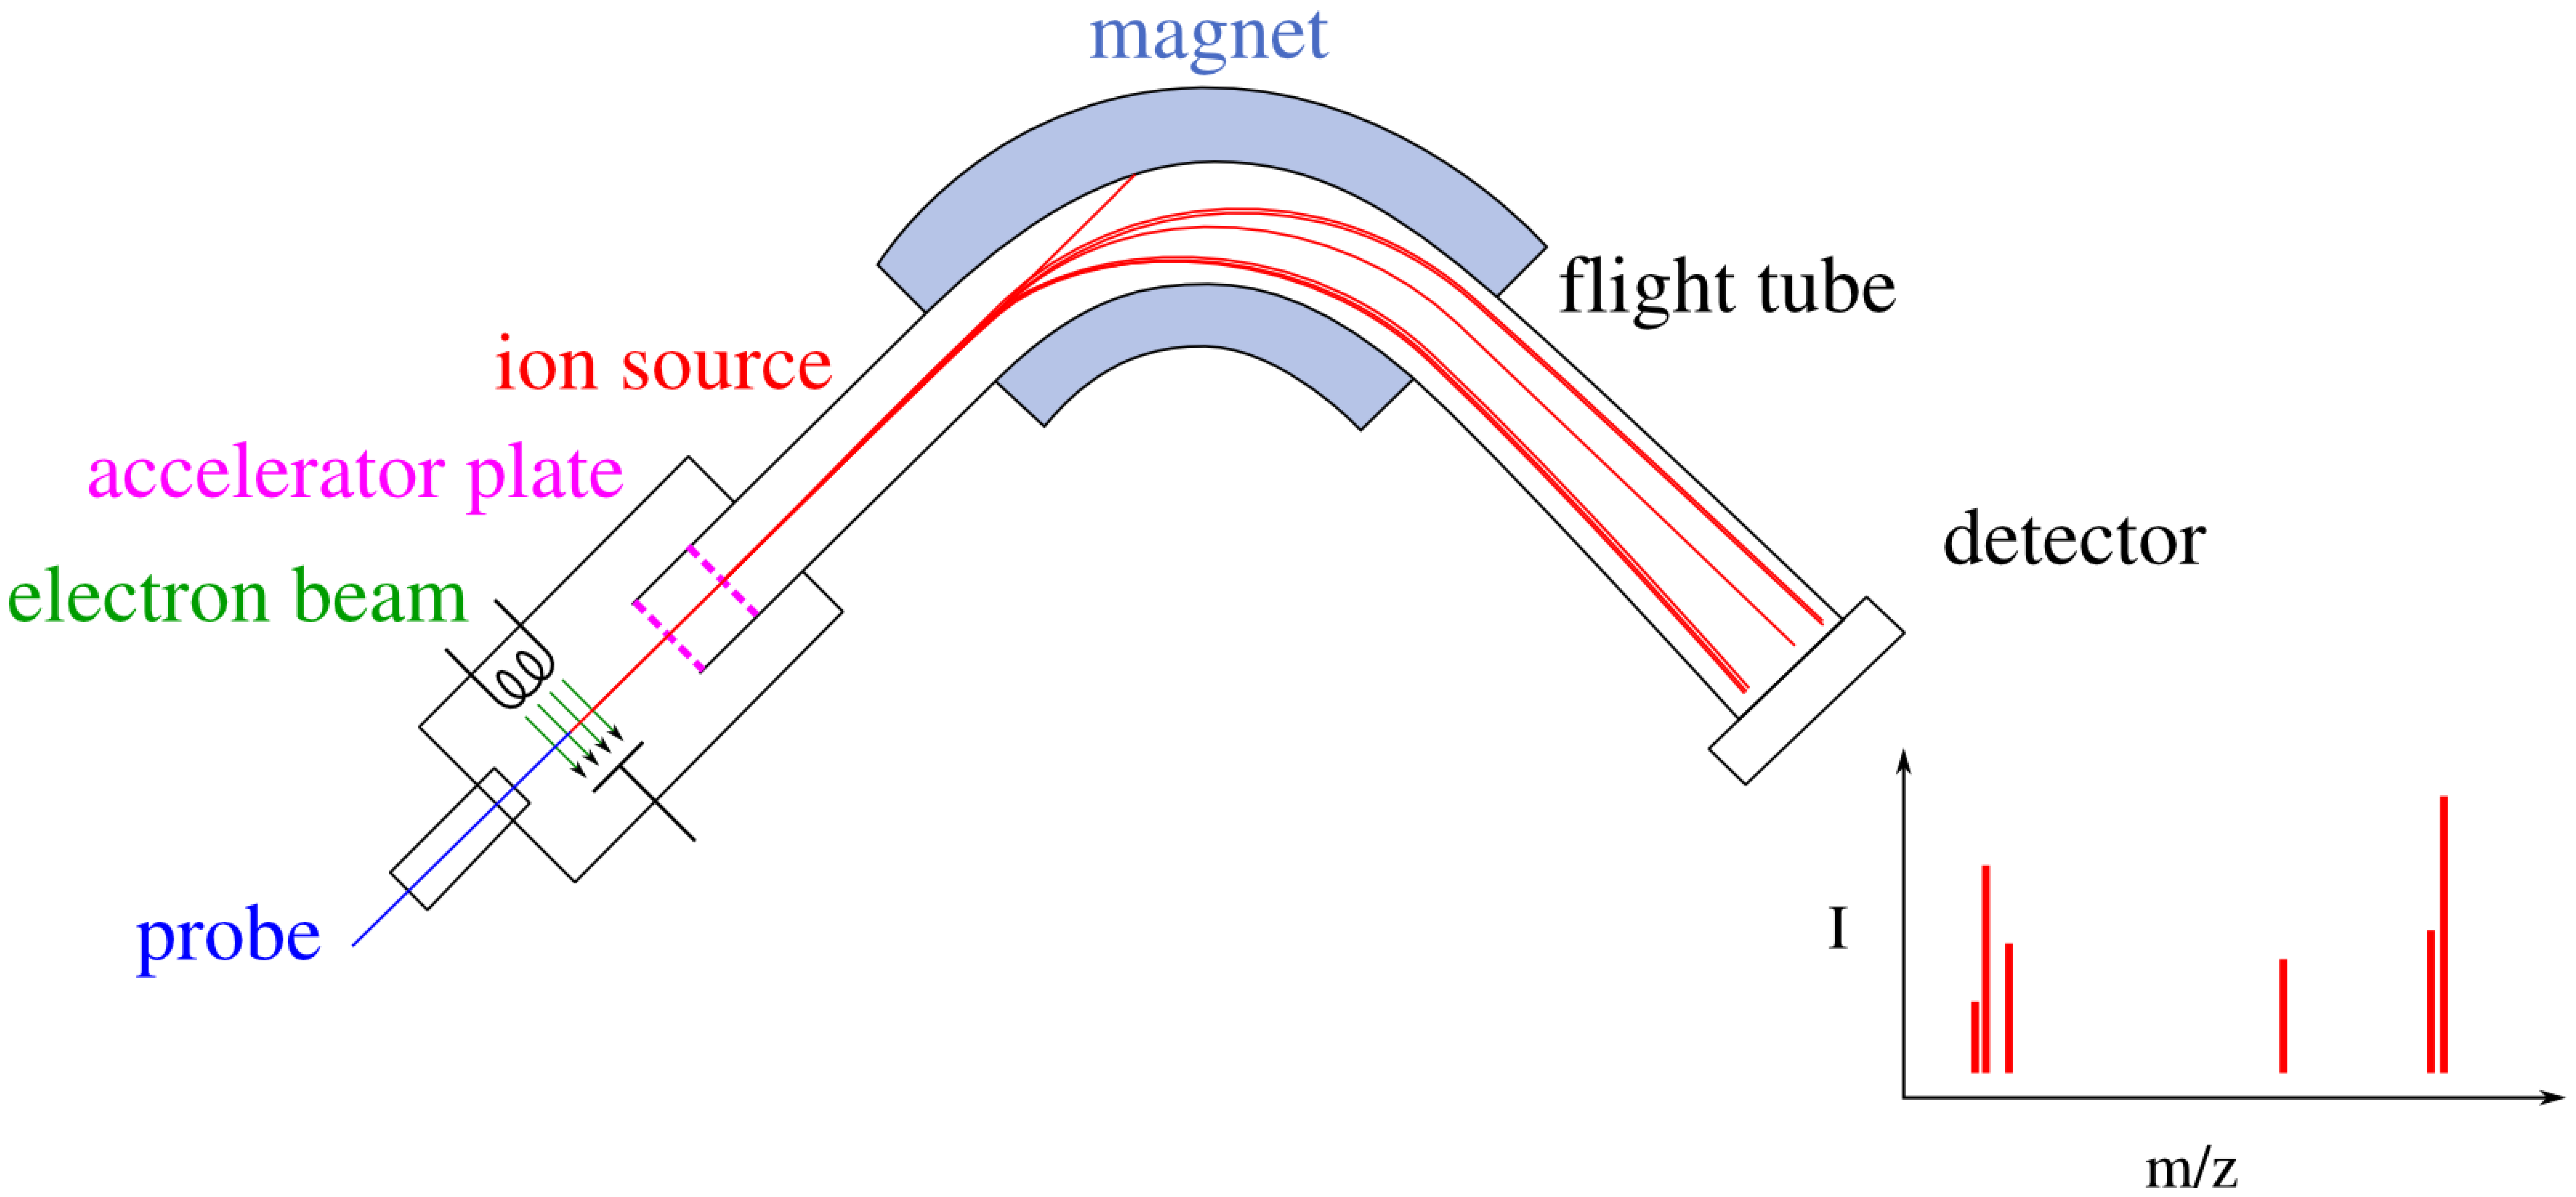
\includegraphics[scale=0.15]{images/MassSpectrometry.eps}
\caption{\footnotesize{
Schematic diagram of a mass spectrometer
}}
\label{fig: schematic diagram mass spectrometer}
\end{figure}

A mass spectrometer consists of three components: an ion source, a mass analyzer, and a detector, as shown in Figure (\ref{fig: schematic diagram mass spectrometer}). 
The ionizer converts the sample (which may be solid, liquid, or gas) into ions by bombarding it with electrons (electron ionization).
Only some of the collisions are energetic enough to knock one or more electrons out of the sample producing positive ions on the gas phase.
This may cause some of the sample's molecules to break into charged fragments.
An extraction system removes ions from the sample, which are then trajected through the mass analyzer.
The differences in masses of the fragments allows the mass analyzer to sort the ions by their mass/charge ratio, by
accelerating them with an electric or magnetic field, until the fragments reach the detector.
Results are displayed a spectrum of the relative abundance of detected ions as a function of the mass/charge ratio into 
a ``stick diagram''.
The atoms or molecules in the sample can be identified by correlating known masses to the identified masses or through a characteristic fragmentation pattern.
In summary, the mass spectrum shows the mass of the ionized molecule and the masses of its corresponding ionic fragments.

When a highly energetic electron hits a neutral molecule, some of its energy is 
transferred to
this molecule. If the transferred energy excess the \textit{ionization energy} (IE) of the neutral molecule, then the 
ionization by ejection of one electron occurs,
generating a molecular ion in an excited state.
\begin{equation}
M+e^{-} \longrightarrow M^{+*} + 2e^-
\end{equation}
This is the most desirable process. However there are several processes in competition that complicate this situation in practice.
Some of them are shown in Figure (\ref{fig: Processes under EI}).
In principle, only unimolecular reactions are possible for the gaseous ions formed under the usual mass spectrometry
operating conditions. 
As the energy of the electrons increases, the number of channels, abundance and
variety of the ionized species will also increase, which gives rise to a fingerprint of the parent molecule's spectrum.

\begin{figure}[ht]
\centering
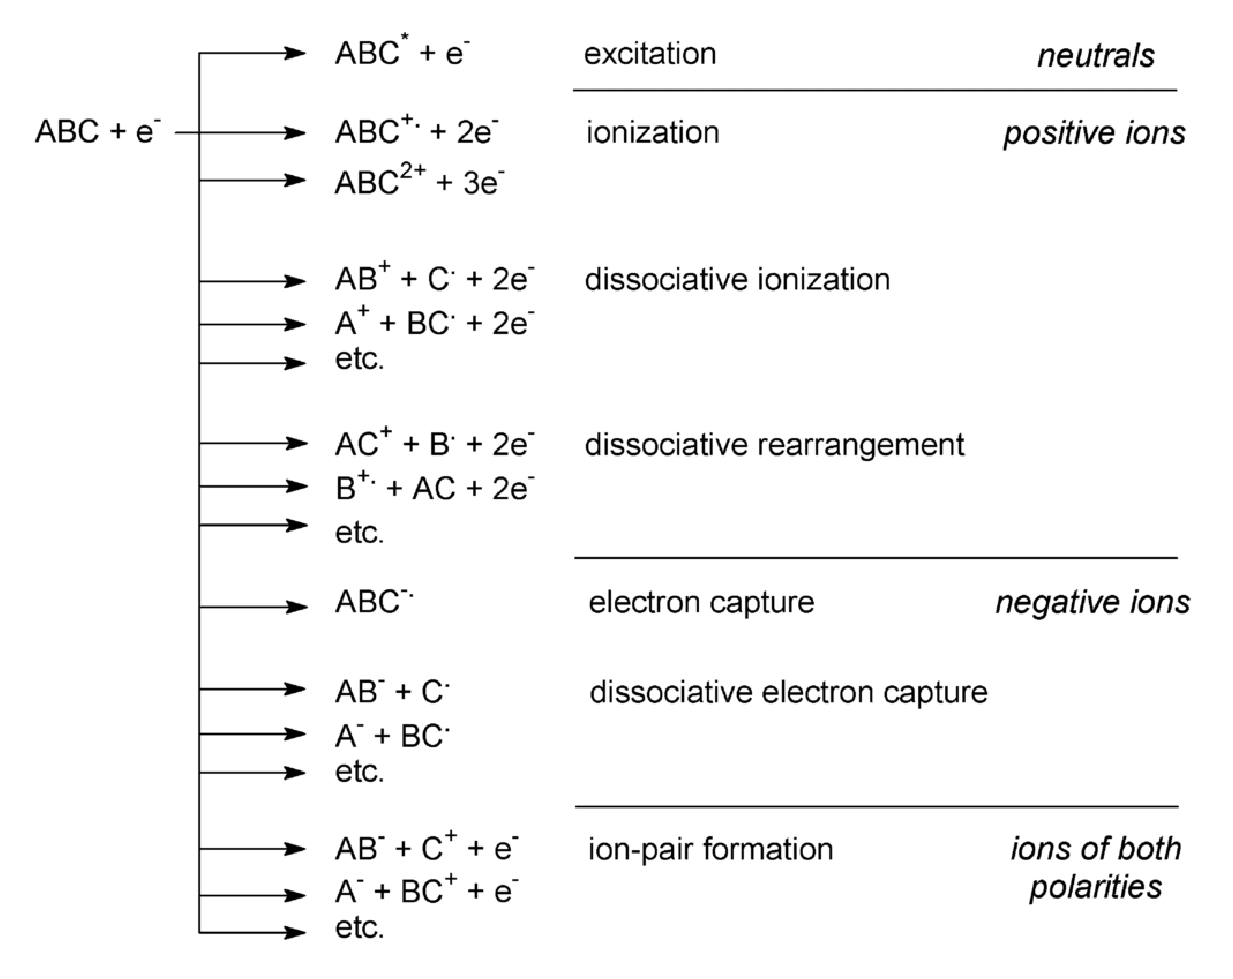
\includegraphics[scale=0.6]{images/processesUnderElectronIonization.eps}
\caption{\footnotesize{
Processes under electron ionization conditions. Taken from: Jürgen H. Gross. Mass Spectrometry. A Textbook. Springer; 2nd ed. 2011 edition. Chapter 2, page 24.
}}
\label{fig: Processes under EI}
\end{figure}

Ionization of the sample molecules with 70 eV electrons produces molecular ions whose internal energy values ($E$)
typically cover a broad range from 0 eV up to 20 eV.
The nature and extent of these reactions depend only on the ion's structure and internal
energy irrespective of the ionization method.

The electron impact ionization of a molecule is a process which takes place in
approximately $10^{-16}$ s and initially yields the exited molecular ion.
The process is much more rapid than the time of one vibration, which is about $10^{-14}$ s. The distances between atoms thus do not change during the
ionization. Thus, this ionization/excitation process can be seen as a vertical transition.
After the ionization, the energy is distributed over the various molecule's degrees of freedom
in a statistical fashion.

The fast exchange of internal energy occurs not only between
the various degrees of freedom of the same electronic state but also between all the degrees
of freedom of all the electronic states. These exchanges lead to the conversion of
electronic energy acquired during ionization into vibrational and rotational energy of the
ground electronic state of the molecular ion.  It can be shown experimentally that the statistical
energy distribution is carried
out within a time span corresponding to a few vibrations, that is less than $10^{-10}$ s. Note that
this time span is very short with respect to the time spent in the spectrometer source, at
least $10^{-7}$ s. Then, fragmentation can be studied independently of the excitation process.
Thus the probabilities of the various possible decompositions
of an ion depend only on its structure and internal energy, and not on the method used for the initial ionization , or 
on the structure of the precursor for, or formation mechanism of, the ion undergoing decomposition.
S. Weerasinghe \textit{et. al.} (\textit{J. Chem. Phys.} \textbf{98} (1993) 4967)
have shown that the dynamical evolution of a complicated many-body system is mainly guided by
the accessible phase-space. Then, statistical mechanics provides the appropriate theoretical framework for
conducting this kind of simulations.

\begin{figure}[h]
\centering
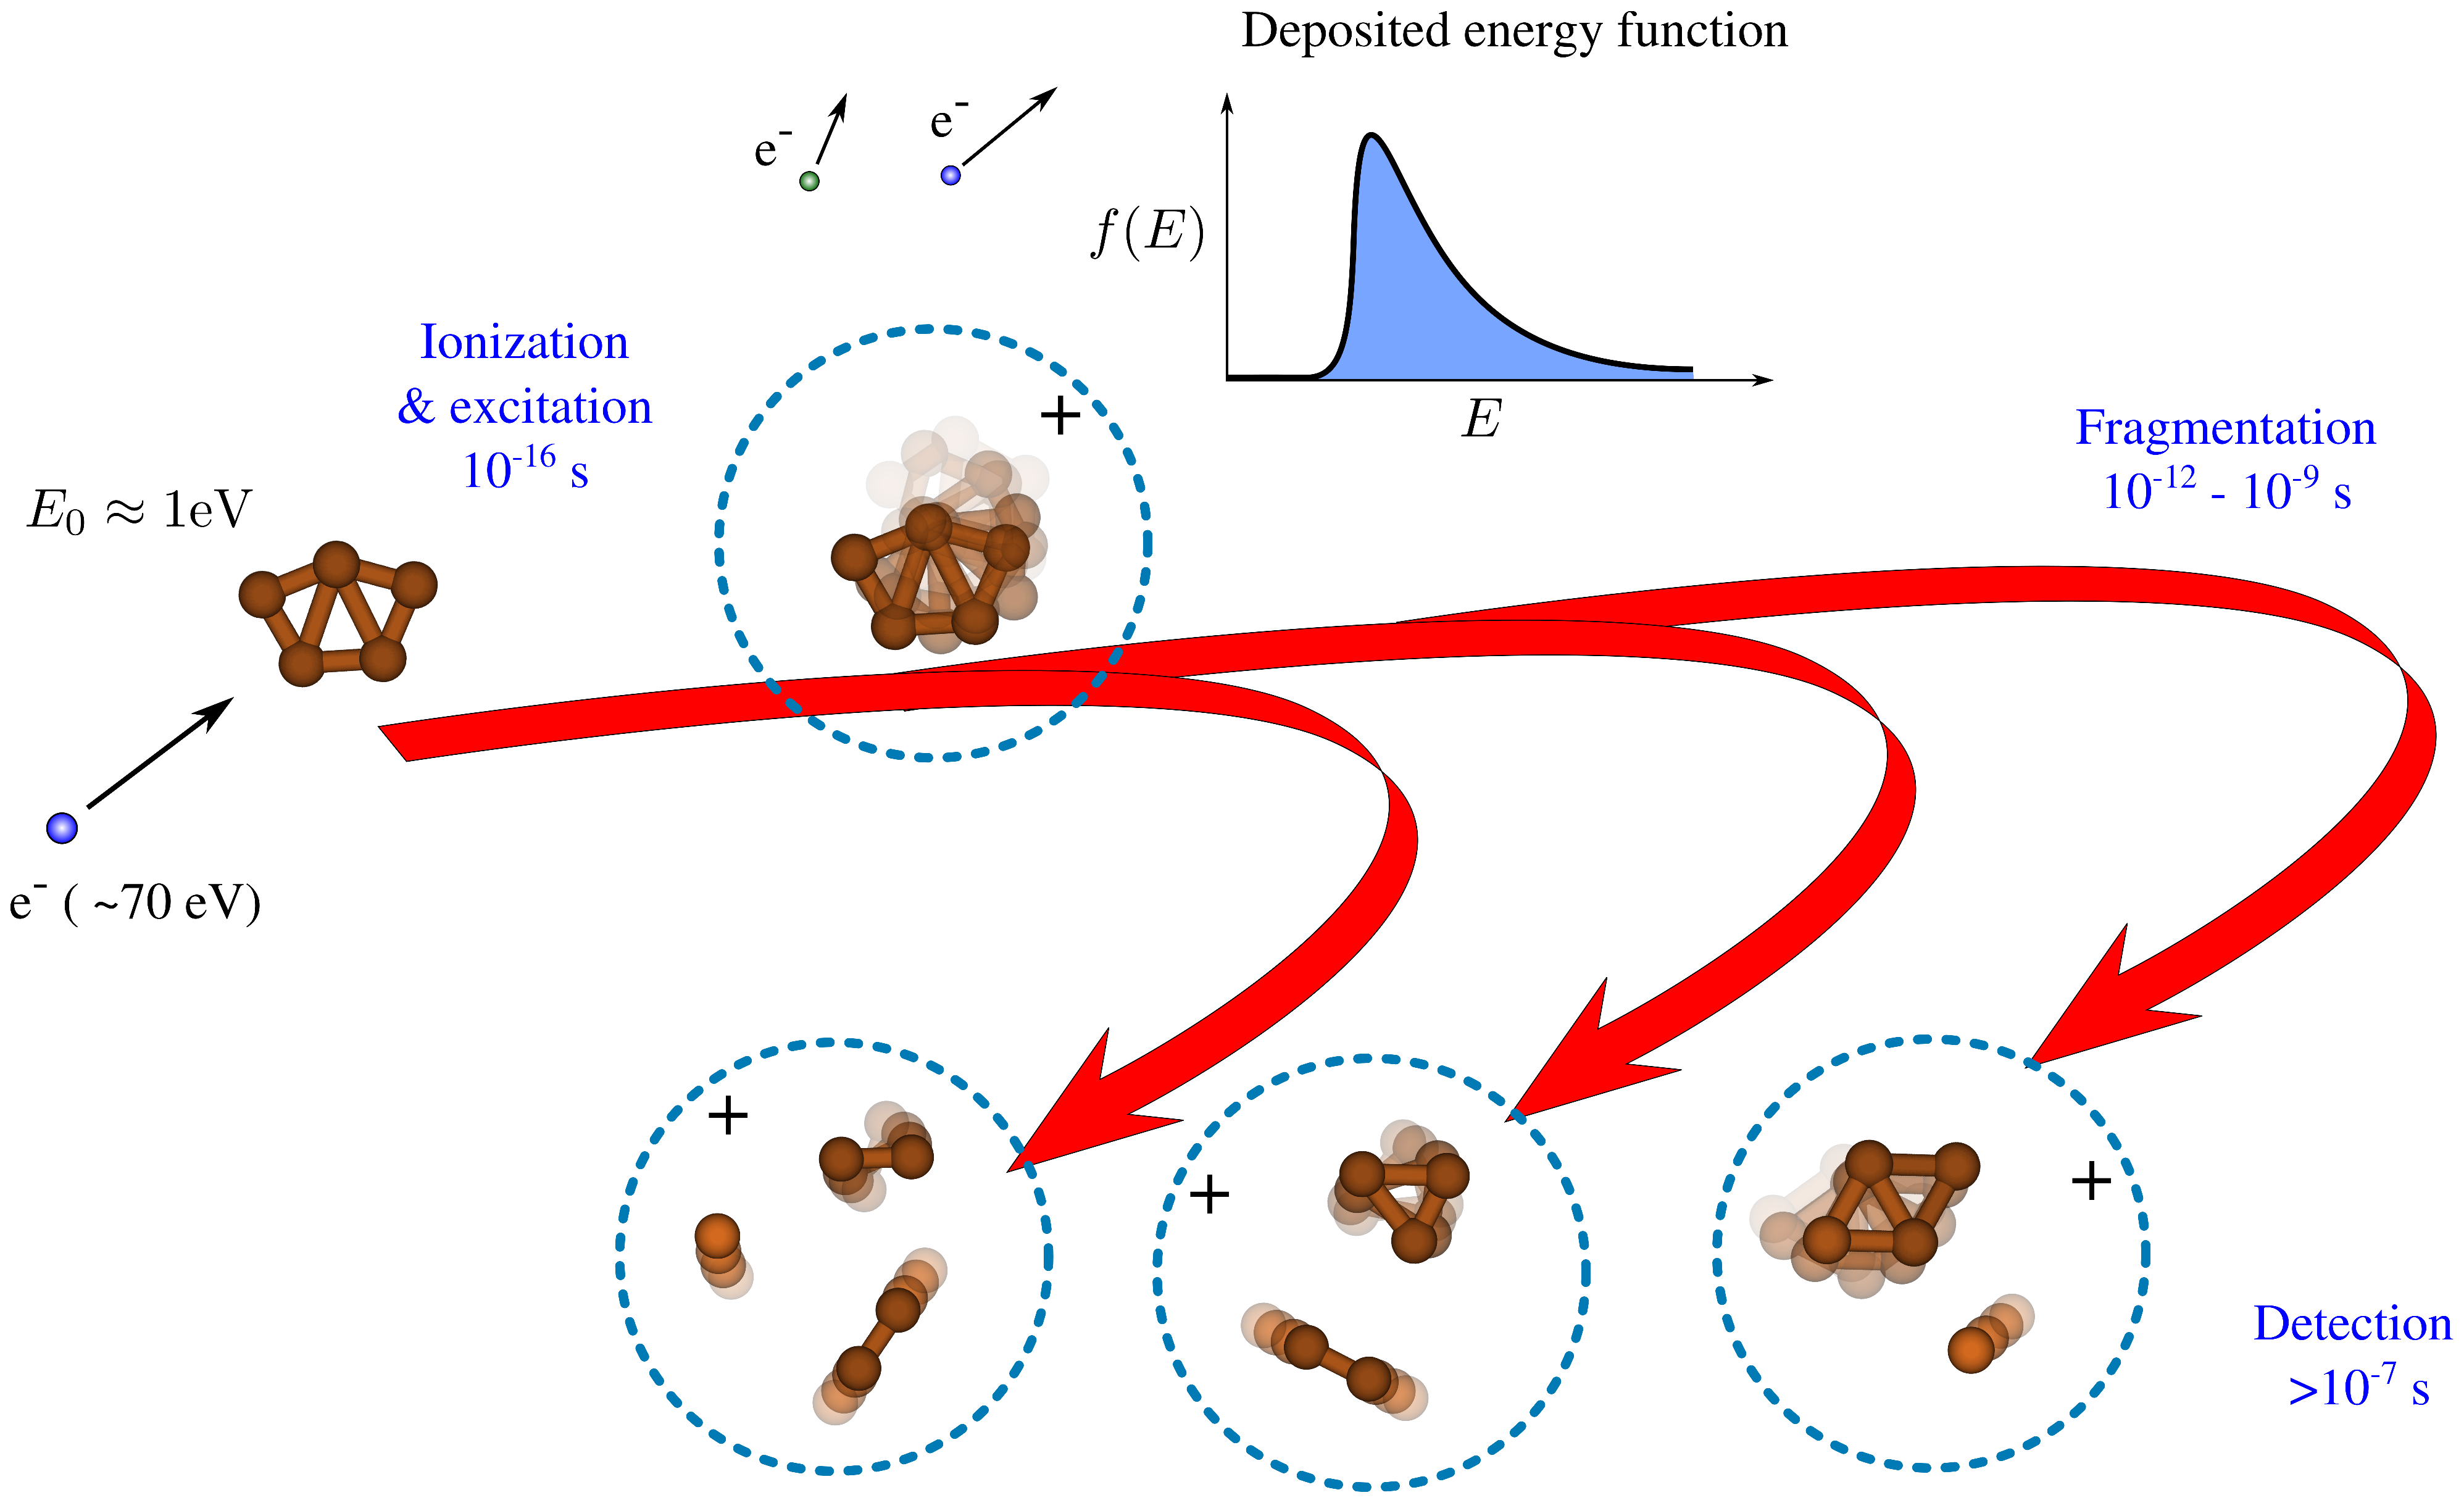
\includegraphics[scale=0.18]{images/fragmentationScheme.eps}
\caption{\footnotesize{
Schematic diagram of the fragmentation process induced by the electron impact ionization
}}
% \label{}
\end{figure}

\section{Basics of Microcanonical Metropolis Monte-Carlo }

The statistical Microcanonical Metropolis Monte-Carlo (M$_3$C) method is a theoretical approach that 
allows to describe the unimolecular decompositions
of ions and hence their mass spectra. A better comprehension of the fragmentation mechanisms is the main goal.
This theoretical description is based on the following premises:
\begin{enumerate}
\item There is no change of position or kinetic energy of the nuclei while the ionization and excitation processes take place ( ``vertical transition'' ).
\item The molecular ion will access to as many low-lying excited electronic states as necessary. Radiationless transitions then will result in
transfer of electronic energy into vibrational, rotational or translational energy.
\item These low-lying excited electronic states will not be repulsive; hence, the molecular ions will not dissociate immediately,
but rather remain together for a time long enough for the excess electronic energy to become randomly distributed over all internal degrees of freedom.

\item The deposited energy on the ion depends only on its structure and the experimental setup details.
Thus, the probabilities of the different decomposition channels will not depend on the method used for the initial ionization.

\item The fragmentation channels are determined by the configuration of maximum entropy which is energetically accessible.
It depends only on its structure and internal energy.
Rearrangements of the ions would occur in the same fashion.
\end{enumerate}

This description is focused on the fragmentation processes itself, irrespective
of the excitation mechanism that leads to fragmentation. Furthermore the initial state of the system corresponds
to an excited molecule where its excess of energy ($E$) is given by an unknown energy deposited function $f(E)$, which contains
all the information about the associated experimental details.
The main information provided for the methodology developed in this work are the breaking-curves. Then, the mass spectrum can be obtained by summing the breaking-down curves over the distribution of internal energy imparted to the molecular ions by the electronic ionization process.

Let's do a short introduction of the statistical theory underlying this implementation.
This tutorial is focused on how to get the mass spectra of two different molecules.

In the theory of thermodynamics several ensembles can be considered. A particular ensemble is defined by a set of magnitudes. In the microcanonical ensemble the physical system under study (atoms, molecules, clusters, spins...) has a fixed energy $E$.

In this ensemble, an isolated system at equilibrium is characterized by its microcanonical entropy, given by the 
Boltzmann's formula  $\mathcal{S}=k_b\ln\Omega(E)$, where the number of accessible micro-states into a semiclassical description
is proportional to the micro-canonical density of states (DOS),
\begin{equation}
\Omega(E)
=
\int
d\mathbf{\Gamma}\,
\mathlarger{\delta}
\Bigl[
\mathscr{H}(\boldsymbol{\Gamma}) - E
\Bigr]
\label{eq: definition of DOS}
\end{equation}
here $\mathscr{H}(\boldsymbol{\Gamma})$ represents the Hamiltonian of the system, and $\boldsymbol{\Gamma}$
its phase space, which consists of all the possible values of position and momentum variables.
It is clear that the most important quantity in the microcanonical description is the DOS.

In our specific case, after some assumptions, Equation (\ref{eq: definition of DOS}) can be factorized as follows:"
\begin{equation}
\Omega(E)
\approx
\frac{1}{\mathcal{N}}
\sum_{i=1}^{N_c}
\sum_{j=1}^{N_v}
\sum_{k=1}^{\mathcal{N}}
\,\,\,\,
\Omega^\prime
\left(
E,\mathbf{c}_i,\mathbf{E}_{v,ij},\boldsymbol{\mathcal{R}}_{ik},\boldsymbol{\theta}_{ik},\mathbf{J}_{ik}
\right)
\label{eq:total dos montecarlo}
\end{equation}
This means that the total DOS can be seen as an average of the \textbf{ instantaneous DOS } (iDOS)
$\Omega^\prime
\left(
E,\boldsymbol{\mathcal{X}}
\right)$
which is a function of the sytem's \textbf{state vector}
\begin{equation}
\boldsymbol{\mathcal{X}}=(\mathbf{c},\mathbf{E}_v,\boldsymbol{\mathcal{R}},\boldsymbol{\theta},\mathbf{J})
\end{equation}
Here $\mathbf{c}$ represents the composition of the system (number of molecules and their identity) and
$\mathbf{E}_v,\boldsymbol{\mathcal{R}},\boldsymbol{\theta},\mathbf{J}$ the
vibrational energy, position (Cartesian coordinates of their centers of mass), orientation and angular momentum
for the complete set of molecules or fragments.

The exact mathematical representation of $\Omega^\prime\left(E,\boldsymbol{\mathcal{X}}\right)$ is not important here, since the most
important point that we have to keep in mind is how to generate the minimum number of state-vectors, in order
to obtain a good approximation for the DOS according to the Equation (\ref{eq:total dos montecarlo}).
Here it is where we take advantage of the stochastic sampling methods. In particular, we use the
Markov Chain Monte Carlo sampling algorithm (see Figure (\ref{fig: schematic diagram of markov chain})).

\begin{figure}[h]
\centering
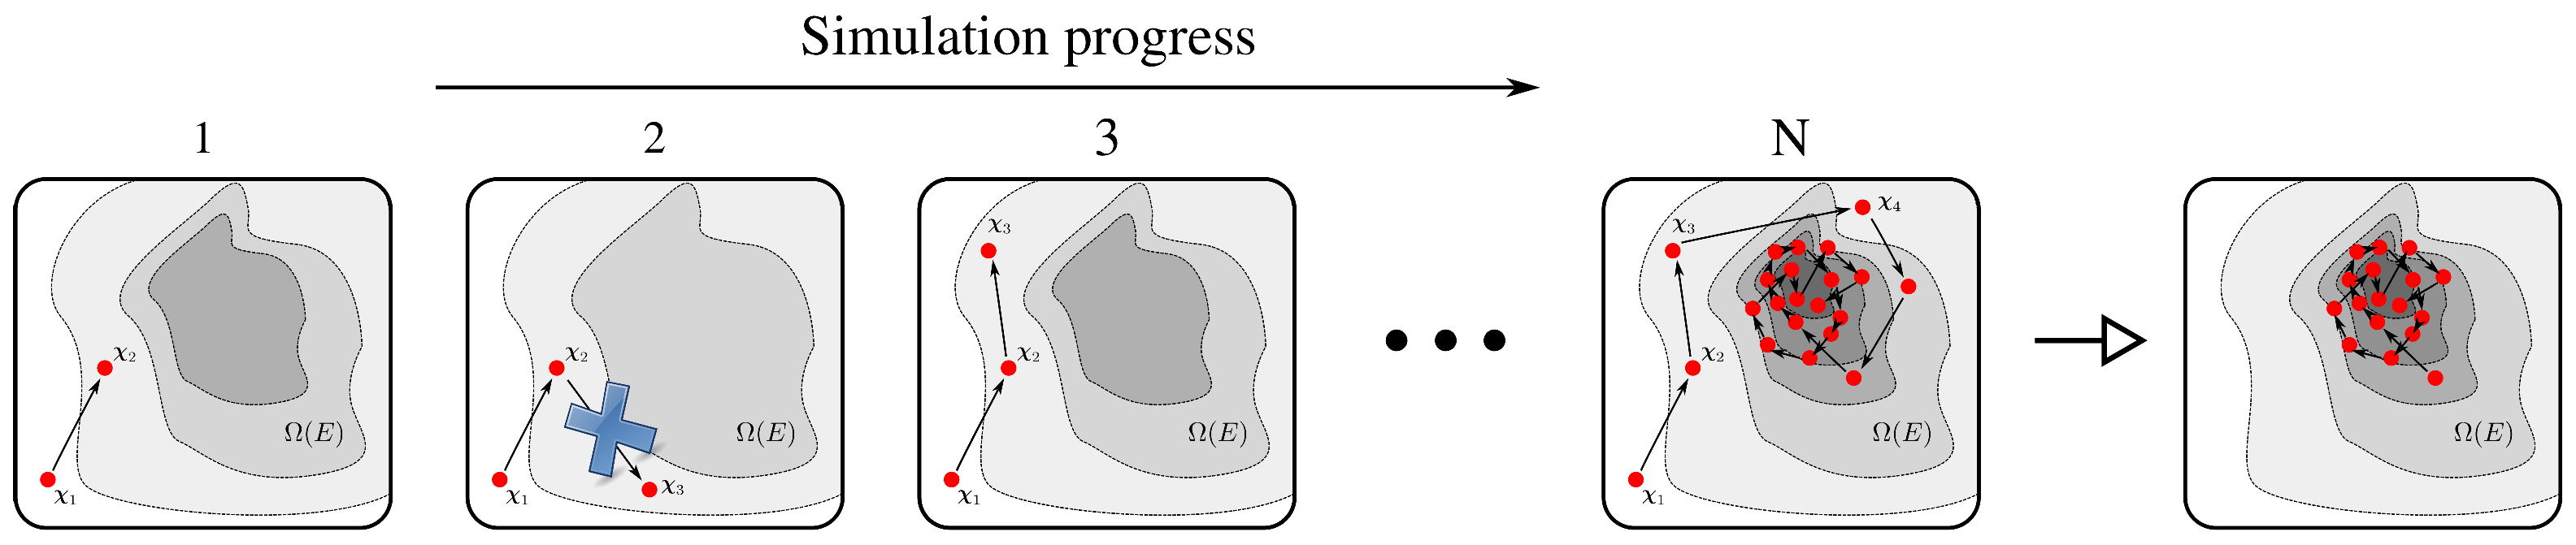
\includegraphics[scale=0.3]{images/stateVectorSearch.eps}
\caption{\footnotesize{
Schematic representation of the $N$-state Markov Chain sampling used to explore the state-vector space $\mathcal{X}$.
}}
\label{fig: schematic diagram of markov chain}
\end{figure}

The microcanonical average of a quantity $f(\boldsymbol{\Gamma})$ is expressed as,
\begin{equation}
\Bigl\langle f(\boldsymbol{\Gamma}) \Bigr\rangle
=
\frac{
\bigintsss d\boldsymbol{\Gamma}\,\,f(\boldsymbol{\Gamma})
}{
\bigintsss d\boldsymbol{\Gamma}
}
\end{equation}
However, several components of the phase-space $\boldsymbol{\Gamma}$
can be integrated out, which allows to express this average in the space of the system's state-vectors
as follows
\begin{equation}
\Bigl\langle f(\boldsymbol{\mathcal{X}}) \Bigr\rangle = \sum_{k=1}^{N}
P(\boldsymbol{\mathcal{X}}_k) f(\boldsymbol{\mathcal{X}}_k),
\label{eq: averages in state vectors}
\end{equation}
where the probability density of finding the system in the configuration $\boldsymbol{\mathcal{X}}_k$ is:
\begin{equation}
P(\boldsymbol{\mathcal{X}}_k)
=
\Omega(E,\boldsymbol{\mathcal{X}}_k)\Bigl/\Omega(E)
\end{equation}
This probability function can be used as the weighting factor in a microcanonical Markov chain Monte Carlo
simulation to calculate averages according to equation (\ref{eq: averages in state vectors}).
In this method we move in small steps
$\{\boldsymbol{\mathcal{X}}_1, \boldsymbol{\mathcal{X}}_2, \cdots, \boldsymbol{\mathcal{X}}_k, \cdots, \boldsymbol{\mathcal{X}}_N\}$
(Markov chain) towards the most important region of the phase space,
\textit{i.e.} highest values for the $\Omega(E,\boldsymbol{\mathcal{X}}_k)$.
In the $k$th-step we generate a candidate $\boldsymbol{\mathcal{X}}_{k+1}$ which will be accepted or rejected depending
of the acceptance ratio $p_E(\boldsymbol{\mathcal{X}}_k\rightarrow\boldsymbol{\mathcal{X}}_{k+1})$, given by
\begin{equation}
p_E(\boldsymbol{\mathcal{X}}_k\rightarrow\boldsymbol{\mathcal{X}}_{k+1})
=
\min\left(
1,
\frac{P(E,\boldsymbol{\mathcal{X}}_{k+1})}{P(E,\boldsymbol{\mathcal{X}}_k)}
\right)
\label{eq: acceptance probability}
\end{equation}
It is important to highlight, that this expression for the acceptance ratio is specially convenient, because
it does not depend on the normalization constant $\Omega(E)$. Then, the acceptance ratio can be simplified to
\begin{equation}
p_E(\boldsymbol{\mathcal{X}}_k\rightarrow\boldsymbol{\mathcal{X}}_{k+1})
=
\min\left(
1,
\frac{\Omega(E,\boldsymbol{\mathcal{X}}_{k+1})}{\Omega(E,\boldsymbol{\mathcal{X}}_k)}
\right)
\end{equation}

At the end of the simulation, after the equilibration of the system (burn-in period), if we generate $N$
randomly state-vectors (accepted or rejected) according to equation (\ref{eq: acceptance probability}), expected values can be approximated by 
a simple arithmetic average
, as follows
\begin{equation}
\Bigl\langle f(\boldsymbol{\mathcal{X}}) \Bigr\rangle = \frac{1}{N}\sum_{k=1}^{N}f(\boldsymbol{\mathcal{X}}_k),
\label{eq: averages in state vectors final}
\end{equation}
where errors in $\langle f(\boldsymbol{\mathcal{X}}) \rangle$ scale as $1/\sqrt{N}$. Figure (\ref{fig: schematic diagram of markov chain})
represents a schematic representation of this algorithm, note the removing of the burn-in period.

In summary, the theoretical description behind this method/implementation is a specific random way to move in the state-vectors space until a
region of maximum entropy is reached, where the physical observables are measured by performing a statistical average 
in this region. In the current version of M$_3$C the available observables includes: channels/species distributions,
energy components distributions, temperature and heat capacity among others. Additionally, by providing a deposited 
energy function $f(E)$
it is possible also to calculate channels' or species' branching ratios and the associated mass spectra.

\section{Goals}

\begin{figure}[h]
\centering
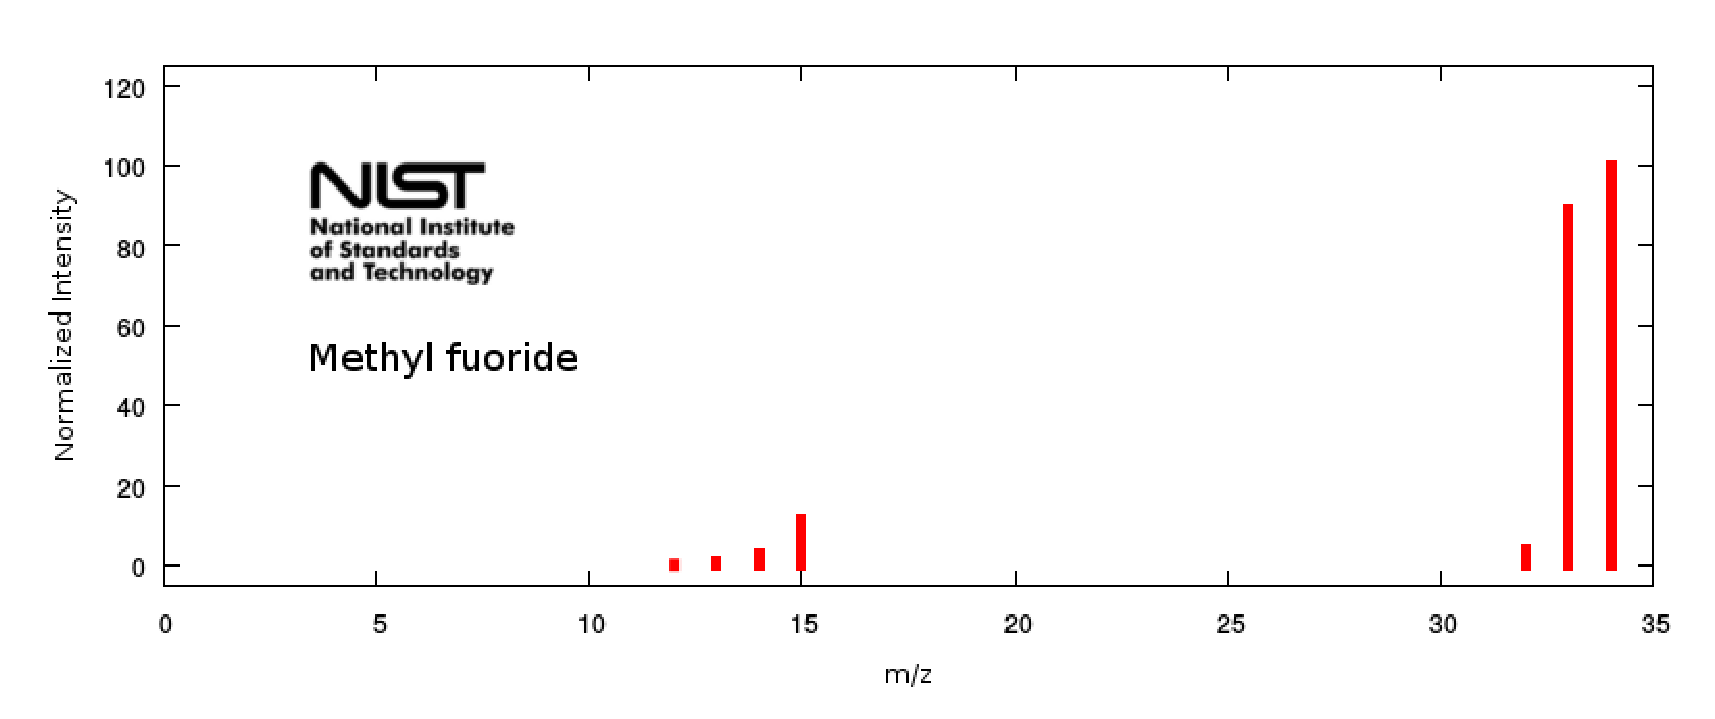
\includegraphics[scale=0.45]{images/NIST-CH3F.eps}
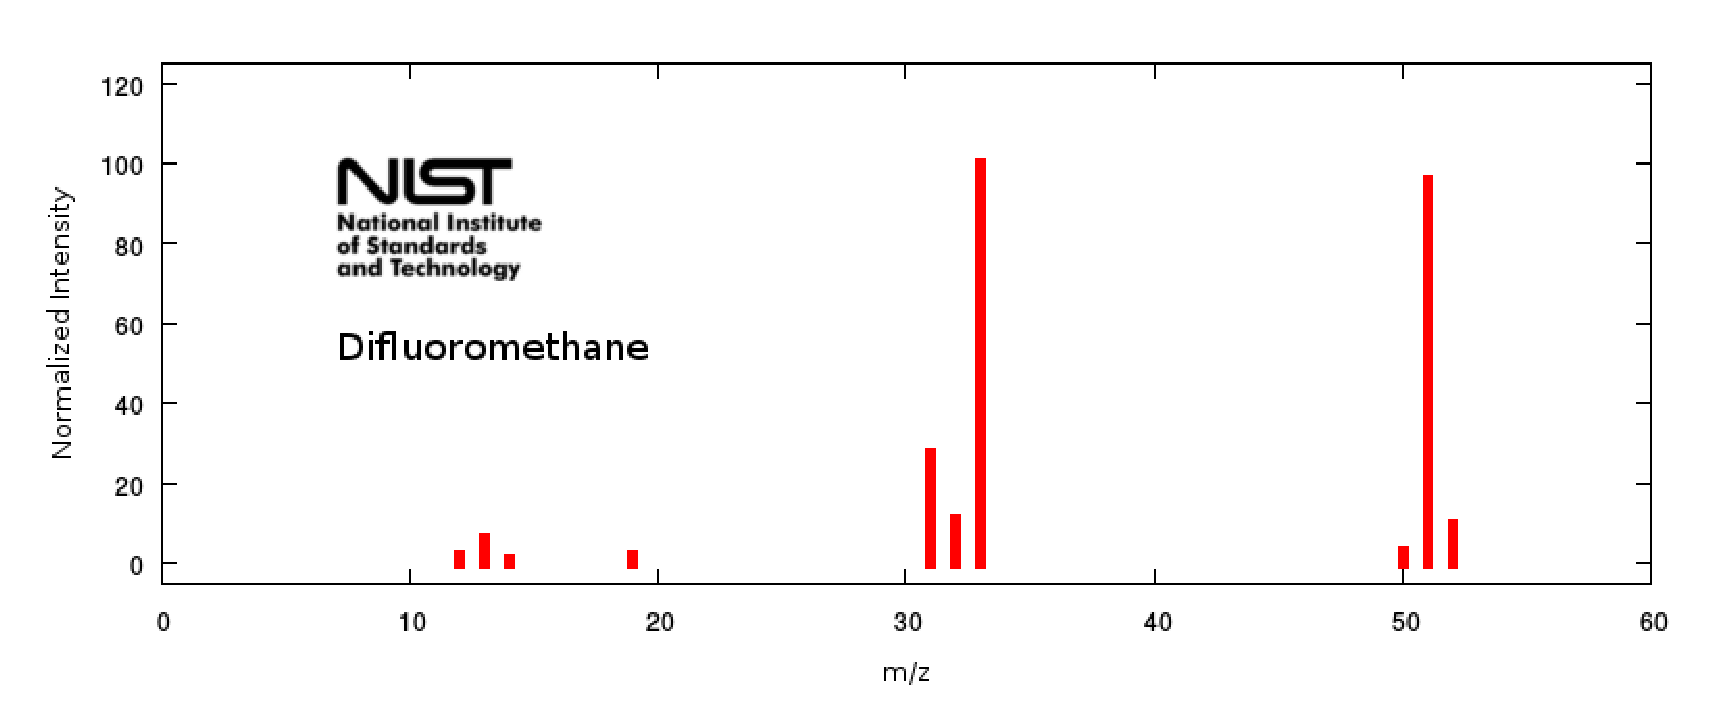
\includegraphics[scale=0.45]{images/NIST-CH2F2.eps}
\caption{\footnotesize{
Data from NIST Standard Reference Database 69: NIST Chemistry WebBook.
NIST Mass Spec Data Center, S.E. Stein, director, "Mass Spectra" in NIST Chemistry WebBook, NIST Standard Reference 
Database Number 69, Eds. P.J. Linstrom and W.G. Mallard, National Institute of Standards and Technology, Gaithersburg 
MD, 20899, http://webbook.nist.gov, (retrieved January 3, 2015). 
}}
\label{fig: experimental mass spectra}
\end{figure}

In this tutorial we will show you how to build a mass spectrum from scratch. The minimum information that \texttt{M3C} needs is 
the electronic energy, molecular geometry and vibrational frequencies for all possible molecules (local minima) which 
are involved in the fragmentation process. As more molecules you consider, better results you will obtain. So, taking 
into account that the most expensive computational part corresponds to obtain these parameters, we will dedicate an 
important part of this tutorial to show, how to use the scripts provided by the M3C program, to carry out this task.

We have chosen two related systems to illustrate how M3C works: fluoromethane (also called methyl fluoride) CH$_3$F and 
difluoromethane CH$_ 2$F$_2$. The experimental mass spectra for these two molecules are shown on the Figure 
(\ref{fig: experimental mass spectra}). The most remarkable difference between them is that in the second one, 
the molecular ion peak does not corresponds to the base peak (the most abundant ion), in contrast with the first one. 
After reading this tutorial you will be able to clarify the origin of this effect.

\section{Example 1: Fluoromethane (guided tour)}

Our main hypothesis is that fragmentation process occurs in two steps:
\begin{equation}
\begin{aligned}
\text{C}\text{H}_3\text{F}(E_0)
+ e^{-}(\varepsilon)
&\rightarrow
\text{C}\text{H}_3\text{F}^+(E_0+E) + 2e^-
\\[4mm]
\text{C}\text{H}_3\text{F}^+(E_0+E)
&\rightarrow
\text{H}_2\text{C}^+ + \text{HF}
\\
&\rightarrow
\text{H}_2 + \text{HCF}^+
\\
&\rightarrow
\text{H} + \text{HC} + \text{HF}^+
\\
&\rightarrow \cdots
\end{aligned}
\end{equation}
The first one corresponds to the
electronic ionization, which leads to the associated cation with an energy excess $E$. $E$ is
distributed according to a specific energy deposited function $f(E)$ which we assume contains all information about
the experimental conditions. The second one is the cation's fragmentation process itself. We suppose
that the first step is much faster that the second one, therefore the measured fragmentation patterns
when the fragments reach the detectors depend mainly on the fragmentation process.
This means, simulating the mass spectrum for the CH$_3$F is equivalent to simulating the fragmentation process
of its cation CH$_3$F$^+$, convoluted by an energy deposited function $f(E)$.

The first step in our simulation is to get all geometries for the possible fragments and their isomers. First we will
make a stochastic search by using a molecular electronic structure code, these calculations will be done by using a
semi empirical method, due its high computational time consuming. Then, the first guess of molecular structures will
be refined at DFT-B3LYP/6-311+G* level of theory. The vibrational frequencies will be obtained at the end by using the
same level of theory. Once all structures and vibrational frequencies are available for all possible fragments, they
will be used to build the M3C input file.

At the end of this document you will find a step-by-step summary without descriptions. We recommend you follow
these steps first and them return to this document to understand their meaning.

\subsection{Stochastic search for isomers}

How many fragments can we get by the fragmentation of the CH$_3$F$^+$ molecule? This is a combinatorial problem which 
is equivalent to get the different combinations of the three elements $\{$H,C,F$\}$ with repetitions (maximum one for
C and F, and three for H). M$_3$C offers an automatic way to calculate it by using the command \texttt{M3C.fragments}, as follows:
\begin{shellexec}
user@hostname\$ M3C.fragments H3,C,F

H, C, F, H2, HC, HF, CF, H3, H2C, H2F, HCF, H3C, H3F, H2CF, H3CF
\end{shellexec}
Fifteen possible fragments are obtained.
Here, we could discard some of them by chemical arguments of stability or based on the peaks which appear in the 
experimental mass spectrum. This could be very important for molecular systems which consist of a vast number of 
particles, because search for isomers it is the most expensive computational part of this methodology. However, we are 
going to continue considering all possible combinations for this system.

Now, it is neccesary to build trial geometries, one for each fragment. To do it you can use any of the free available
molecular editors in the web, as \textbf{avogadro}\footnote{http://avogadro.cc/wiki/Main\_Page}, \textbf{molden} 
\footnote{http://www.cmbi.ru.nl/molden/}, \textbf{pymol} \footnote{http://www.pymol.org/}, among others.
Figure (\ref{fig: trial geometries for fluoromethane}) shows the trial geometries we used. Note that these geometries
do not necessarily correspond to stable molecules, these only are an initial guess. These geometries are stored
in the directory \texttt{init}.

% ---------------------------------------------------------------------------------------------
% This table has been generated with the following command:
% ../getGifTable.sh 8
% ---------------------------------------------------------------------------------------------

\begin{figure}[ht]
\centering
\begin{tabular}{|
>{\centering\arraybackslash}p{1.6cm}|
>{\centering\arraybackslash}p{1.6cm}|
>{\centering\arraybackslash}p{1.6cm}|
>{\centering\arraybackslash}p{1.6cm}|
>{\centering\arraybackslash}p{1.6cm}|
>{\centering\arraybackslash}p{1.6cm}|
>{\centering\arraybackslash}p{1.6cm}|
>{\centering\arraybackslash}p{1.6cm}|
}
\hline

\includegraphics[scale=0.3]{images/tableInitial/H.eps} \ttiny{1 \hspace{5pt} H} &

\includegraphics[scale=0.3]{images/tableInitial/C.eps} \ttiny{2 \hspace{5pt} C} &

\includegraphics[scale=0.3]{images/tableInitial/F.eps} \ttiny{3 \hspace{5pt} F} &

\includegraphics[scale=0.3]{images/tableInitial/H2.eps} \ttiny{4 \hspace{5pt} H2} &

\includegraphics[scale=0.3]{images/tableInitial/HC.eps} \ttiny{5 \hspace{5pt} HC} &

\includegraphics[scale=0.3]{images/tableInitial/HF.eps} \ttiny{6 \hspace{5pt} HF} &
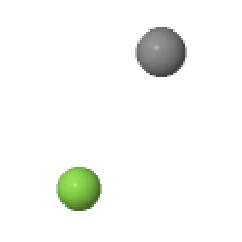
\includegraphics[scale=0.3]{images/tableInitial/CF.eps} \ttiny{7 \hspace{5pt} CF} &

\includegraphics[scale=0.3]{images/tableInitial/H3.eps} \ttiny{8 \hspace{5pt} H3}
\\\hline

\includegraphics[scale=0.3]{images/tableInitial/H2C.eps} \ttiny{9 \hspace{5pt} H2C} &
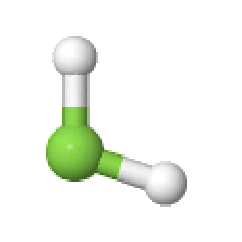
\includegraphics[scale=0.3]{images/tableInitial/H2F.eps} \ttiny{10 \hspace{5pt} H2F} &
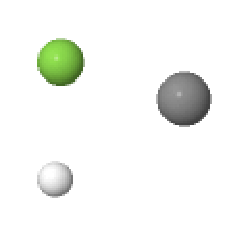
\includegraphics[scale=0.3]{images/tableInitial/HCF.eps} \ttiny{11 \hspace{5pt} HCF} &
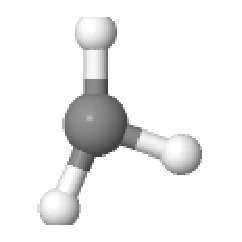
\includegraphics[scale=0.3]{images/tableInitial/H3C.eps} \ttiny{12 \hspace{5pt} H3C} &
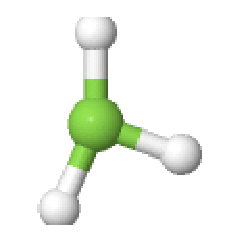
\includegraphics[scale=0.3]{images/tableInitial/H3F.eps} \ttiny{13 \hspace{5pt} H3F} &

\includegraphics[scale=0.3]{images/tableInitial/H2CF.eps} \ttiny{14 \hspace{5pt} H2CF} &

\includegraphics[scale=0.3]{images/tableInitial/H3CF.eps} \ttiny{15 \hspace{5pt} H3CF} 
\\\cline{1-7}
\end{tabular}
\caption{\footnotesize{
Trial geometries used to represent the possible fragments in the fragmentation of the CH$_3$F$^+$ molecule.
}}
\label{fig: trial geometries for fluoromethane}
\end{figure}

% ---------------------------------------------------------------------------------------------

The procedure can begin with any structure for the fragments. It is submitted to GAMESS\footnote{http://www.msg.ameslab.gov/gamess/} program optimization.
The minimum energy structure obtained is then stored. The initial structure (without optimization) is then subject to an operation called a \textit{kick},
each atom is moved a random distance in a random direction. The constraints are the maximum distance the atoms are going to be moved and the maximum radius allowed of the system $R_{\text{sys}}$ (\texttt{systemRadius}), to generate a configuration where their atoms are non-overlapping. Each atom is kicked to a position within a sphere of radius $R$ (\texttt{randomWalkStepRadius}) around
its initial position, where $R$ is the maximum kick distance. After all the atoms are randomly moved in this way, quantum mechanical optimization
is carried out again. This algorithm is typically referred to as the \textbf{random walker algorithm}. Figure (\ref{fig: random walkers}) shows an example of the trajectories obtained by a system of three particles after thousands steps.

\begin{figure}[h]
\centering
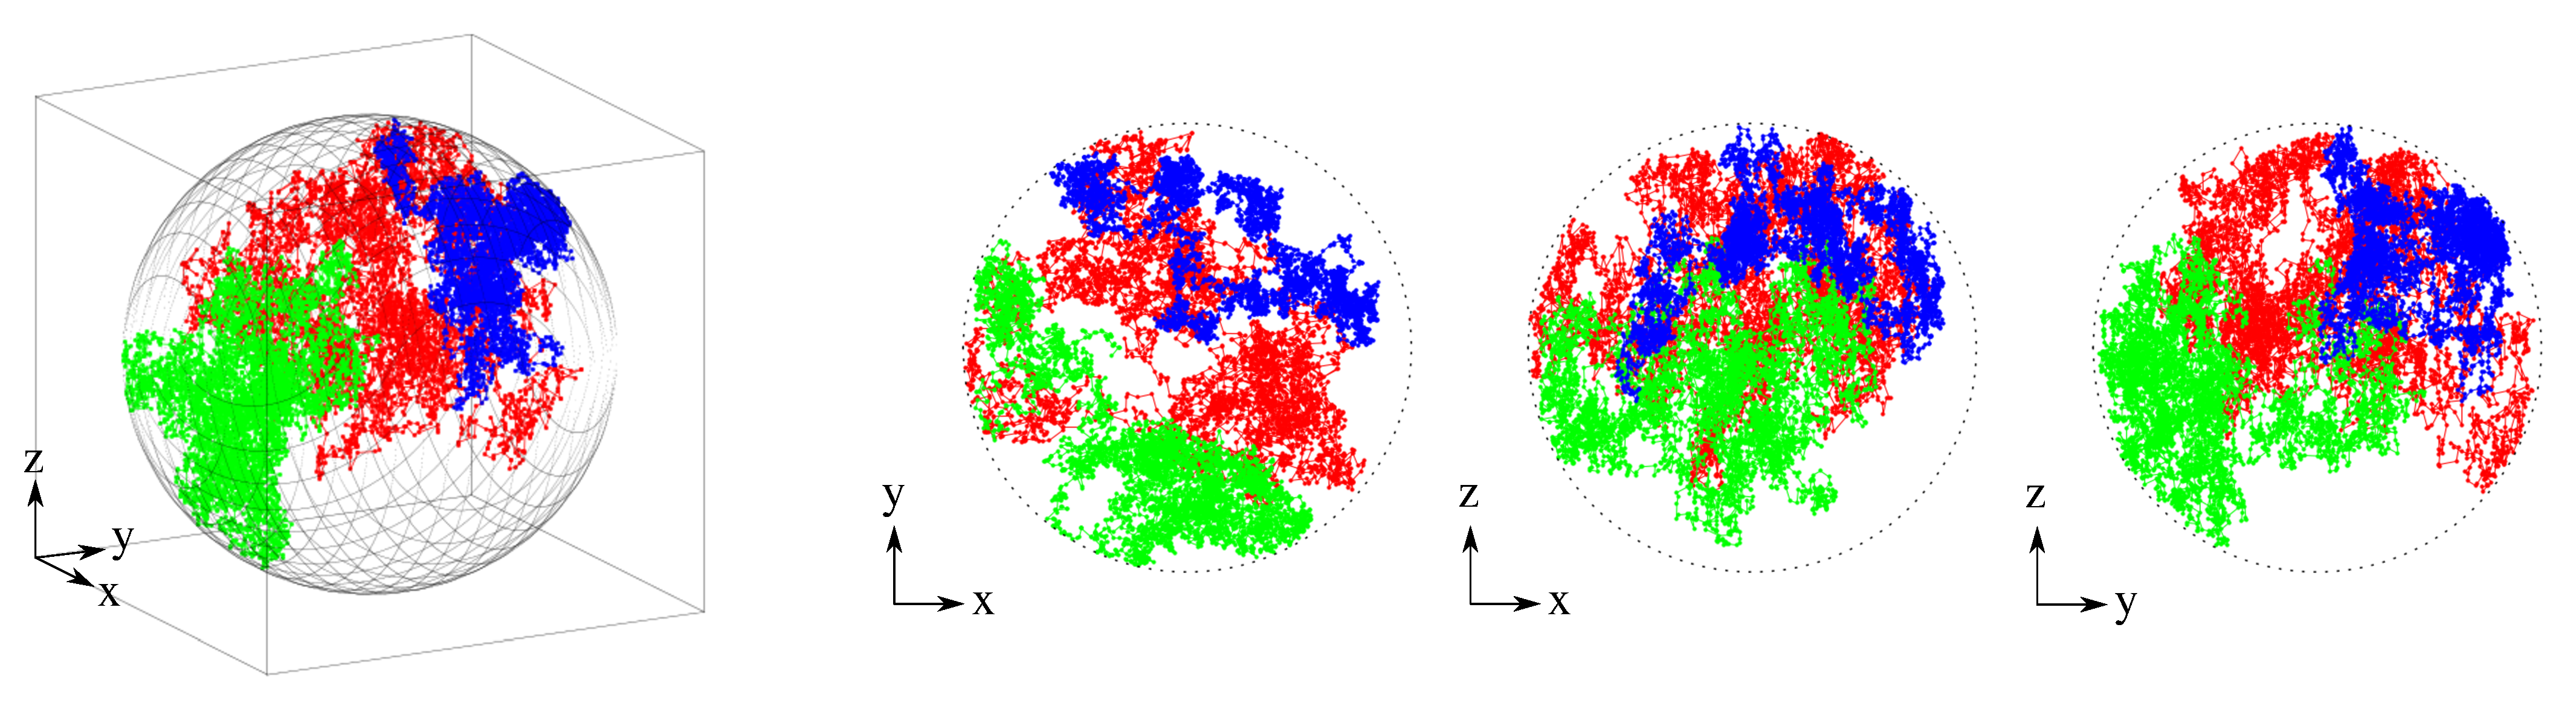
\includegraphics[scale=0.2]{images/randomWalkers.eps}
\caption{\footnotesize{
Example of the trajectories followed by 3 particles with different massses by using the random walker algorithm described in the text.
}}
\label{fig: random walkers}
\end{figure}

For each step, there are two possible results: the structure can go back to some previous state or it can go to a different structure. Then at the end
of the algorithm, a filter removes duplicate isomers. If this procedure is repeated enough times, eventually all isomeric structures for the molecule will be found.

The controlling parameter in the operation of stochastic searching is the size of the kick. Small kicks will result in return to the kicked isomer. It is easy to start with a small kick and gradually increase it to see when isomerization starts to occur with some reasonable probability. This probability will become larger with further increase of the kick size. With very large kicks, molecules often break into separate pieces. These pieces do not usually come back together into
the optimization process to form bonds and the optimization usually stops at some point. With experience, one can fairly readily find the range of kick size, which gives a reasonable probability of isomerization and yet does not cause fragmentation to occur too frequently.

M3C offers a way to execute the above explained algorithm in an automatic way by interfacing with GAMESS through the command \texttt{M3C-gamess.geniso}.
\texttt{M3C-gamess.geniso} requires three files as parameters: 1) A GAMESS template to control the geometry optimizations, 2) A M3C input file
to control each step of the geometries' random search, and 3) and a file containing the charges, multiplicities and initial geometries to use.
We will describe briefly each one:

\begin{itemize}

\item
\textbf{GAMESS template}.
First we need a GAMESS template for the optimization processes like the following. For each step, variables \texttt{@CHARGE}, \texttt{@MULT} and 
\texttt{@GEOMETRY} will be substituted by the corresponding charge, multiplicity and by the geometry block respectively.
In this example geometry optimization is carried out at the PM3 semiempirical level.

\begin{bifile}[caption=\footnotesize GAMESS template for geometry optimization at PM3 level (pm3.optg-GAMESS.inp)]
 $contrl runtyp=optimize icharg=@CHARGE mult=@MULT $end
 $basis gbasis=pm3 $end
 $statpt projct=.f. nstep=50 $end
 $system timlim=600000 memory=2500000 $end
 $data
 pm3
 c1
 @GEOMETRY
 $end
\end{bifile}

\item
\textbf{M3C input file}.
This input file will control the generation of the next non-overlapping geometry.
The input file is divided in blocks, in the GOPTIONS block you can change the system radius and the maximum kick distance. The REACTOR block defines a 
geometric-translational operation (\texttt{type=T}). The reactor will read the geometry from products.xyz, it will modify it in a random way and it will save 
it by using the same file name. FRAGMENTS\_DATABASE block defines the parts of the molecule that will be moved, in this case it will correspond to the atoms, 
however, as it will be shown later, it also can be molecules. M3C is case sensitive for input files, comments start with \# and lenght units in angstroms.

\begin{bifile}[caption=\footnotesize M3C input file for random walker algorithm (reactorT.m3c)]
BEGIN GOPTIONS
        systemRadius = 2.0
        overlappingRadius = 0.3
        
        randomWalkStepRadius = 1.5
        useRandomWalkers = TRUE
END GOPTIONS

BEGIN REACTOR
        type = T

        reactives = file:products.xyz
        excitationEnergy = 10.0

        geomProductsFile = products.xyz
END REACTOR

BEGIN FRAGMENTS_DATABASE
        #---------------------------------------------------------
        # Label    Z  M  L  SYM         geomFile            Eelec 
        #                                   Angs               eV 
        #---------------------------------------------------------
              C    0  1  0    0           C.xyz         0.000000
              H    0  1  0    0           H.xyz         0.000000
              F    0  1  0    0           F.xyz         0.000000
        #---------------------------------------------------------
END FRAGMENTS_DATABASE
\end{bifile}

\item
\textbf{Configuration file}.
This file presents a simple table format. The first column is the file with the initial trial geometry, the second one is the
charge (\texttt{@CHARGE}) and the last one the multiplicity (\texttt{@MULT}). Each row represents an electronic configuration
for a chosen stoichiometry as given in the XYZ file. In this file, we have included only fragments with charge up to one and
the lowest multiplicity state, in order to obtain better results. It could include states with higher multiplicity.

\begin{bifile}[caption=\footnotesize Configuration file (fragments.inp)]
#-----------------------
# XYZfile  charge  mult
#-----------------------
    F.xyz     0      2
    C.xyz     0      1
   CF.xyz     0      2
    H.xyz     0      2
   HF.xyz     0      1
   HC.xyz     0      2
  HCF.xyz     0      1
   H2.xyz     0      1
  H2F.xyz     0      2
  H2C.xyz     0      1
 H2CF.xyz     0      2
   H3.xyz     0      2
  H3F.xyz     0      1
  H3C.xyz     0      2

    F.xyz     1      1
    C.xyz     1      2
   CF.xyz     1      1
    H.xyz     1      0
   HF.xyz     1      2
   HC.xyz     1      1
  HCF.xyz     1      2
   H2.xyz     1      2
  H2F.xyz     1      1
  H2C.xyz     1      2
 H2CF.xyz     1      1
   H3.xyz     1      1
  H3F.xyz     1      2
  H3C.xyz     1      1
 H3CF.xyz     1      2
\end{bifile}

\end{itemize}
Once the above files have been prepared, the command \texttt{M3C-gamess.geniso} can be executed as follows
\begin{shellexec}
user@hostname\$ ls
CH3F+.m3c  fragments.inp  init

user@hostname\$ M3C-gamess.geniso fragments.inp ../pm3.optg-GAMESS.inp ../reactorT.m3c 10 init results

Running:    F,   C,   CF,   H,   HF,  HC, HCF,  H2 ... OK   Time elapsed: 0h  3m 59s
Running:  H2F, H2C, H2CF,  H3,  H3F, H3C,   F,   C ... OK   Time elapsed: 0h 13m 55s
Running:   CF,   H,   HF,  HC,  HCF,  H2, H2F, H2C ... OK   Time elapsed: 0h  7m 49s
Running: H2CF,  H3,  H3F, H3C, H3CF                ... OK   Time elapsed: 0h 13m  8s
                                                                   Total: 0h 38m 51s
user@hostname\$ ls
CH3F+.m3c  fragments.inp  init  results
\end{shellexec}
In this example, ten random configurations have been generated for each stoichiometry, and all successful optimizations have been stored into directory 
\texttt{results}. Geometry files are coded with the format \texttt{<label>.q<charge>.m<mult>.xyz}.
Total elapsed time was around forty minutes.
\begin{shellexec}
user@hostname\$ cd results
user@hostname\$ ls

CF.q0.m2-1.xyz    H3CF.q1.m2-1.xyz  H3F.q1.m2-6.xyz    history-C.q1.m2*     history-H3.q0.m2*
CF.q1.m1-1.xyz    H3CF.q1.m2-2.xyz  H3.q0.m2-1.xyz     history-F.q0.m2*     history-H3.q1.m1*
...
H2.q0.m1-10.xyz   H3F.q1.m2-2.xyz   history-CF.q1.m1*  history-H3F.q0.m1*
H2.q1.m2-10.xyz   H3F.q1.m2-3.xyz   history-C.q0.m1*   history-H3F.q1.m2*
\end{shellexec}
All optimized geometries can be easily visualized by using the command \texttt{M3C.viewXYZ} as follows
\begin{shellexec}
user@hostname\$ M3C.viewXYZ
CF.q0.m2-1.xyz ... OK
CF.q1.m1-1.xyz ... OK
...
H.q0.m2-1.xyz ... OK
H.q1.m0-1.xyz ... OK

user@hostname\$ gwenview .
\end{shellexec}
where one should get a diagram like the one shown in Figure (\ref{fig:geometries after M3C.geniso}).

% ---------------------------------------------------------------------------------------------
% This table has been generated with the following command:
% ../getGifTable.sh 8 11,12,13,18,20,21,23,25,26,27,28,29,30,31,32,33,34
% ---------------------------------------------------------------------------------------------

\begin{figure}[ht]
\centering
\begin{tabular}{|
>{\centering\arraybackslash}p{1.6cm}|
>{\centering\arraybackslash}p{1.6cm}|
>{\centering\arraybackslash}p{1.6cm}|
>{\centering\arraybackslash}p{1.6cm}|
>{\centering\arraybackslash}p{1.6cm}|
>{\centering\arraybackslash}p{1.6cm}|
>{\centering\arraybackslash}p{1.6cm}|
>{\centering\arraybackslash}p{1.6cm}|
}
\hline
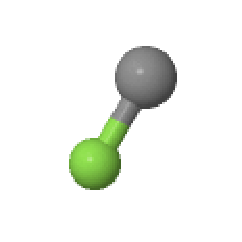
\includegraphics[scale=0.3]{images/table1/CF.q0.m2-1.eps} \ttiny{1 \hspace{5pt} CF.q0.m2-1} &
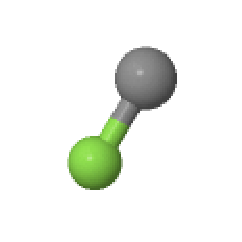
\includegraphics[scale=0.3]{images/table1/CF.q1.m1-1.eps} \ttiny{2 \hspace{5pt} CF.q1.m1-1} &

\includegraphics[scale=0.3]{images/table1/C.q0.m1-1.eps} \ttiny{3 \hspace{5pt} C.q0.m1-1} &

\includegraphics[scale=0.3]{images/table1/C.q1.m2-1.eps} \ttiny{4 \hspace{5pt} C.q1.m2-1} &

\includegraphics[scale=0.3]{images/table1/F.q0.m2-1.eps} \ttiny{5 \hspace{5pt} F.q0.m2-1} &

\includegraphics[scale=0.3]{images/table1/F.q1.m1-1.eps} \ttiny{6 \hspace{5pt} F.q1.m1-1} &
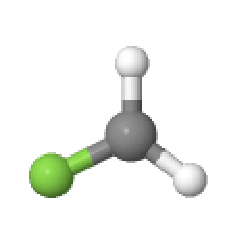
\includegraphics[scale=0.3]{images/table1/H2CF.q0.m2-1.eps} \ttiny{7 \hspace{5pt} H2CF.q0.m2-1} &
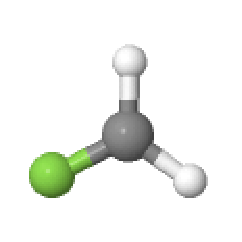
\includegraphics[scale=0.3]{images/table1/H2CF.q1.m1-1.eps} \ttiny{8 \hspace{5pt} H2CF.q1.m1-1} 
\\\hline
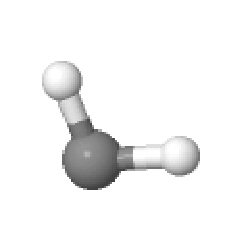
\includegraphics[scale=0.3]{images/table1/H2C.q0.m1-1.eps} \ttiny{9 \hspace{5pt} H2C.q0.m1-1} &
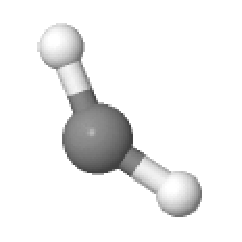
\includegraphics[scale=0.3]{images/table1/H2C.q1.m2-1.eps} \ttiny{10 \hspace{5pt} H2C.q1.m2-1} &

\includegraphics[scale=0.3]{images/table1/H2F.q0.m2-10.eps} \textcolor{red}{\ttiny{11 
\hspace{5pt}H2F.q0.m2-10}} &
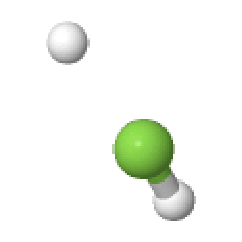
\includegraphics[scale=0.3]{images/table1/H2F.q0.m2-1.eps} \textcolor{red}{\ttiny{12 
\hspace{5pt}H2F.q0.m2-1}} &

\includegraphics[scale=0.3]{images/table1/H2F.q0.m2-9.eps} \textcolor{red}{\ttiny{13 
\hspace{5pt}H2F.q0.m2-9}} &
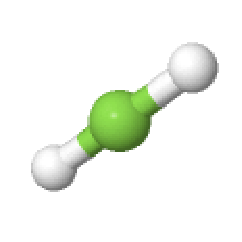
\includegraphics[scale=0.3]{images/table1/H2F.q1.m1-10.eps} \ttiny{14 \hspace{5pt} H2F.q1.m1-10} &
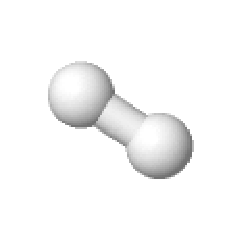
\includegraphics[scale=0.3]{images/table1/H2.q0.m1-10.eps} \ttiny{15 \hspace{5pt} H2.q0.m1-10} &

\includegraphics[scale=0.3]{images/table1/H2.q1.m2-10.eps} \ttiny{16 \hspace{5pt} H2.q1.m2-10} 
\\\hline
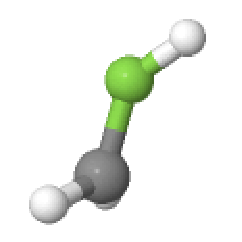
\includegraphics[scale=0.3]{images/table1/H3CF.q1.m2-1.eps} \ttiny{17 \hspace{5pt} H3CF.q1.m2-1} &
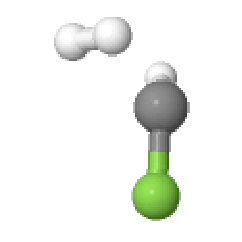
\includegraphics[scale=0.3]{images/table1/H3CF.q1.m2-2.eps} \textcolor{red}{\ttiny{18 
\hspace{5pt}H3CF.q1.m2-2}} &

\includegraphics[scale=0.3]{images/table1/H3C.q0.m2-10.eps} \ttiny{19 \hspace{5pt} H3C.q0.m2-10} &
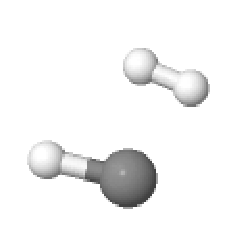
\includegraphics[scale=0.3]{images/table1/H3C.q0.m2-3.eps} \textcolor{red}{\ttiny{20 
\hspace{5pt}H3C.q0.m2-3}} &
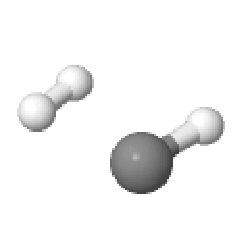
\includegraphics[scale=0.3]{images/table1/H3C.q0.m2-4.eps} \textcolor{red}{\ttiny{21 
\hspace{5pt}H3C.q0.m2-4}} &
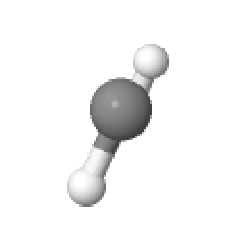
\includegraphics[scale=0.3]{images/table1/H3C.q0.m2-8.eps} \ttiny{22 \hspace{5pt} H3C.q0.m2-8} &
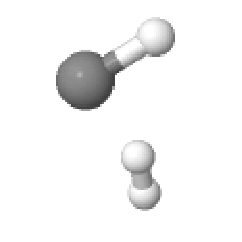
\includegraphics[scale=0.3]{images/table1/H3C.q1.m1-10.eps} \textcolor{red}{\ttiny{23 
\hspace{5pt}H3C.q1.m1-10}} &
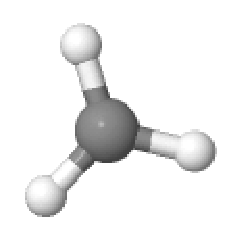
\includegraphics[scale=0.3]{images/table1/H3C.q1.m1-1.eps} \ttiny{24 \hspace{5pt} H3C.q1.m1-1} 
\\\hline

\includegraphics[scale=0.3]{images/table1/H3C.q1.m1-3.eps} \textcolor{red}{\ttiny{25 
\hspace{5pt}H3C.q1.m1-3}} &

\includegraphics[scale=0.3]{images/table1/H3C.q1.m1-4.eps} \textcolor{red}{\ttiny{26 
\hspace{5pt}H3C.q1.m1-4}} &
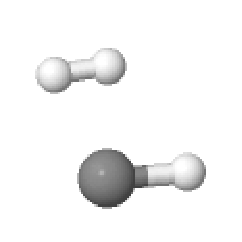
\includegraphics[scale=0.3]{images/table1/H3C.q1.m1-9.eps} \textcolor{red}{\ttiny{27 
\hspace{5pt}H3C.q1.m1-9}} &

\includegraphics[scale=0.3]{images/table1/H3F.q0.m1-1.eps} \textcolor{red}{\ttiny{28 
\hspace{5pt}H3F.q0.m1-1}} &
\includegraphics[scale=0.3]{images/table1/H3F.q0.m1-2.eps} \textcolor{red}{\ttiny{29 
\hspace{5pt}H3F.q0.m1-2}} &
\includegraphics[scale=0.3]{images/table1/H3F.q1.m2-1.eps} \textcolor{red}{\ttiny{30 
\hspace{5pt}H3F.q1.m2-1}} &
\includegraphics[scale=0.3]{images/table1/H3F.q1.m2-2.eps} \textcolor{red}{\ttiny{31 
\hspace{5pt}H3F.q1.m2-2}} &
\includegraphics[scale=0.3]{images/table1/H3F.q1.m2-3.eps} \textcolor{red}{\ttiny{32 
\hspace{5pt}H3F.q1.m2-3}} 
\\\hline
\includegraphics[scale=0.3]{images/table1/H3F.q1.m2-6.eps} \textcolor{red}{\ttiny{33 
\hspace{5pt}H3F.q1.m2-6}} &
\includegraphics[scale=0.3]{images/table1/H3.q0.m2-1.eps} \textcolor{red}{\ttiny{34 
\hspace{5pt}H3.q0.m2-1}} &
\includegraphics[scale=0.3]{images/table1/H3.q0.m2-2.eps} \ttiny{35 \hspace{5pt} H3.q0.m2-2} &
\includegraphics[scale=0.3]{images/table1/H3.q0.m2-3.eps} \ttiny{36 \hspace{5pt} H3.q0.m2-3} &
\includegraphics[scale=0.3]{images/table1/H3.q0.m2-4.eps} \ttiny{37 \hspace{5pt} H3.q0.m2-4} &
\includegraphics[scale=0.3]{images/table1/H3.q0.m2-7.eps} \ttiny{38 \hspace{5pt} H3.q0.m2-7} &
\includegraphics[scale=0.3]{images/table1/H3.q1.m1-10.eps} \ttiny{39 \hspace{5pt} H3.q1.m1-10} &
\includegraphics[scale=0.3]{images/table1/HCF.q0.m1-1.eps} \ttiny{40 \hspace{5pt} HCF.q0.m1-1} 
\\\hline
\includegraphics[scale=0.3]{images/table1/HCF.q1.m2-1.eps} \ttiny{41 \hspace{5pt} HCF.q1.m2-1} &
\includegraphics[scale=0.3]{images/table1/HC.q0.m2-10.eps} \ttiny{42 \hspace{5pt} HC.q0.m2-10} &
\includegraphics[scale=0.3]{images/table1/HC.q1.m1-10.eps} \ttiny{43 \hspace{5pt} HC.q1.m1-10} &
\includegraphics[scale=0.3]{images/table1/HF.q0.m1-10.eps} \ttiny{44 \hspace{5pt} HF.q0.m1-10} &
\includegraphics[scale=0.3]{images/table1/HF.q1.m2-10.eps} \ttiny{45 \hspace{5pt} HF.q1.m2-10} &
\includegraphics[scale=0.3]{images/table1/H.q0.m2-1.eps} \ttiny{46 \hspace{5pt} H.q0.m2-1} &
\includegraphics[scale=0.3]{images/table1/H.q1.m0-1.eps} \ttiny{47 \hspace{5pt} H.q1.m0-1} 
\\\cline{1-7}
\end{tabular}
\caption{\footnotesize{
First set of molecules obtained by the random-walkers algorithm, as implemented in \texttt{M3C-gamess.geniso} 
command.
}}
\label{fig:geometries after M3C.geniso}
\end{figure}

% ---------------------------------------------------------------------------------------------

As it is possible to appreciate in Figure (\ref{fig:geometries after M3C.geniso}),
there are molecules separated into two or more pieces. Such structures were not rejected by the program automatically. 
So, we have to remove these molecules by hand. The molecules that have been 
removed appear highlighted in red. After that, we obtain the set of molecules shown in Figure 
(\ref{fig:geometries after M3C.geniso final}).

% ---------------------------------------------------------------------------------------------
% This table has been generated with the following command:
% ../getGifTable.sh 8
% ---------------------------------------------------------------------------------------------

\begin{figure}[ht]
\centering
\begin{tabular}{|
>{\centering\arraybackslash}p{1.6cm}|
>{\centering\arraybackslash}p{1.6cm}|
>{\centering\arraybackslash}p{1.6cm}|
>{\centering\arraybackslash}p{1.6cm}|
>{\centering\arraybackslash}p{1.6cm}|
>{\centering\arraybackslash}p{1.6cm}|
>{\centering\arraybackslash}p{1.6cm}|
>{\centering\arraybackslash}p{1.6cm}|
}
\hline
\includegraphics[scale=0.3]{images/table2/CF.q0.m2-1.eps} \ttiny{1 \hspace{5pt} CF.q0.m2-1} &
\includegraphics[scale=0.3]{images/table2/CF.q1.m1-1.eps} \ttiny{2 \hspace{5pt} CF.q1.m1-1} &
\includegraphics[scale=0.3]{images/table2/C.q0.m1-1.eps} \ttiny{3 \hspace{5pt} C.q0.m1-1} &
\includegraphics[scale=0.3]{images/table2/C.q1.m2-1.eps} \ttiny{4 \hspace{5pt} C.q1.m2-1} &
\includegraphics[scale=0.3]{images/table2/F.q0.m2-1.eps} \ttiny{5 \hspace{5pt} F.q0.m2-1} &
\includegraphics[scale=0.3]{images/table2/F.q1.m1-1.eps} \ttiny{6 \hspace{5pt} F.q1.m1-1} &
\includegraphics[scale=0.3]{images/table2/H2CF.q0.m2-1.eps} \ttiny{7 \hspace{5pt} H2CF.q0.m2-1} &
\includegraphics[scale=0.3]{images/table2/H2CF.q1.m1-1.eps} \ttiny{8 \hspace{5pt} H2CF.q1.m1-1} 
\\\hline
\includegraphics[scale=0.3]{images/table2/H2C.q0.m1-1.eps} \ttiny{9 \hspace{5pt} H2C.q0.m1-1} &
\includegraphics[scale=0.3]{images/table2/H2C.q1.m2-1.eps} \ttiny{10 \hspace{5pt} H2C.q1.m2-1} &
\includegraphics[scale=0.3]{images/table2/H2F.q1.m1-10.eps} \ttiny{11 \hspace{5pt} H2F.q1.m1-10} &
\includegraphics[scale=0.3]{images/table2/H2.q0.m1-10.eps} \ttiny{12 \hspace{5pt} H2.q0.m1-10} &
\includegraphics[scale=0.3]{images/table2/H2.q1.m2-10.eps} \ttiny{13 \hspace{5pt} H2.q1.m2-10} &
\includegraphics[scale=0.3]{images/table2/H3CF.q1.m2-1.eps} \ttiny{14 \hspace{5pt} H3CF.q1.m2-1} &
\includegraphics[scale=0.3]{images/table2/H3C.q0.m2-10.eps} \ttiny{15 \hspace{5pt} H3C.q0.m2-10} &
\includegraphics[scale=0.3]{images/table2/H3C.q1.m1-1.eps} \ttiny{16 \hspace{5pt} H3C.q1.m1-1} 
\\\hline
\includegraphics[scale=0.3]{images/table2/H3.q0.m2-2.eps} \ttiny{17 \hspace{5pt} H3.q0.m2-2} &
\includegraphics[scale=0.3]{images/table2/H3.q0.m2-4.eps} \ttiny{18 \hspace{5pt} H3.q0.m2-4} &
\includegraphics[scale=0.3]{images/table2/H3.q0.m2-7.eps} \ttiny{19 \hspace{5pt} H3.q0.m2-7} &
\includegraphics[scale=0.3]{images/table2/H3.q1.m1-10.eps} \ttiny{20 \hspace{5pt} H3.q1.m1-10} &
\includegraphics[scale=0.3]{images/table2/HCF.q0.m1-1.eps} \ttiny{21 \hspace{5pt} HCF.q0.m1-1} &
\includegraphics[scale=0.3]{images/table2/HCF.q1.m2-1.eps} \ttiny{22 \hspace{5pt} HCF.q1.m2-1} &
\includegraphics[scale=0.3]{images/table2/HC.q0.m2-10.eps} \ttiny{23 \hspace{5pt} HC.q0.m2-10} &
\includegraphics[scale=0.3]{images/table2/HC.q1.m1-10.eps} \ttiny{24 \hspace{5pt} HC.q1.m1-10} 
\\\hline
\includegraphics[scale=0.3]{images/table2/HF.q0.m1-10.eps} \ttiny{25 \hspace{5pt} HF.q0.m1-10} &
\includegraphics[scale=0.3]{images/table2/HF.q1.m2-10.eps} \ttiny{26 \hspace{5pt} HF.q1.m2-10} &
\includegraphics[scale=0.3]{images/table2/H.q0.m2-1.eps} \ttiny{27 \hspace{5pt} H.q0.m2-1} &
\includegraphics[scale=0.3]{images/table2/H.q1.m0-1.eps} \ttiny{28 \hspace{5pt} H.q1.m0-1} 
\\\cline{1-4}
\end{tabular}
\caption{\footnotesize{
Filtered set of molecules obtained by the random-walkers algorithm with $N=10$ trials, after removal of molecules 
separated into two or more pieces.
}}
\label{fig:geometries after M3C.geniso final}
\end{figure}

% ---------------------------------------------------------------------------------------------

For each stoichiometry, we do not know how many isomers exist in advance. Then, one could
increase the number of the steps in the random-walkers algorithm, in order to verify that the number of 
isomers not change. Specifically we use fifty steps with the following command,

\begin{shellexec}
user@hostname\$ M3C-gamess.geniso fragments.inp ../pm3.optg-GAMESS.inp ../reactorT.m3c 50 init results

Running:    F,   C,   CF,   H,   HF,  HC, HCF,  H2 ... OK   Time elapsed: 0h 23m  4s
Running:  H2F, H2C, H2CF,  H3,  H3F, H3C,   F,   C ... OK   Time elapsed: 1h 21m 24s
Running:   CF,   H,   HF,  HC,  HCF,  H2, H2F, H2C ... OK   Time elapsed: 0h 41m 38s
Running: H2CF,  H3,  H3F, H3C, H3CF                ... OK   Time elapsed: 0h 57m 33s
                                                                   Total: 3h 23m 39s
\end{shellexec}
Total elapsed time was around three hours and a half ( \textit{i.e.} it scales approximately linearly). The final set of
molecules we obtained after filtering
are show in Figure \ref{fig:geometries after M3C.geniso final N 50}. By using 50 steps,
it has emerged one more isomer for the H2CF.q0.m2 and H2CF.q1.m1, H3CF.q1.m2 and HCF.q1.m2 configurations.
We will continue our exercise taking this last set of molecules.

% ---------------------------------------------------------------------------------------------
% This table has been generated with the following command:
% ../getGifTable.sh 8
% ---------------------------------------------------------------------------------------------

\begin{figure}[h]
\centering
\begin{tabular}{|
>{\centering\arraybackslash}p{1.6cm}|
>{\centering\arraybackslash}p{1.6cm}|
>{\centering\arraybackslash}p{1.6cm}|
>{\centering\arraybackslash}p{1.6cm}|
>{\centering\arraybackslash}p{1.6cm}|
>{\centering\arraybackslash}p{1.6cm}|
>{\centering\arraybackslash}p{1.6cm}|
>{\centering\arraybackslash}p{1.6cm}|
}
\hline
\includegraphics[scale=0.3]{images/tableN50/CF.q0.m2-10.eps} \ttiny{1 \hspace{5pt} CF.q0.m2-10} &
\includegraphics[scale=0.3]{images/tableN50/CF.q1.m1-10.eps} \ttiny{2 \hspace{5pt} CF.q1.m1-10} &
\includegraphics[scale=0.3]{images/tableN50/C.q0.m1-1.eps} \ttiny{3 \hspace{5pt} C.q0.m1-1} &
\includegraphics[scale=0.3]{images/tableN50/C.q1.m2-1.eps} \ttiny{4 \hspace{5pt} C.q1.m2-1} &
\includegraphics[scale=0.3]{images/tableN50/F.q0.m2-1.eps} \ttiny{5 \hspace{5pt} F.q0.m2-1} &
\includegraphics[scale=0.3]{images/tableN50/F.q1.m1-1.eps} \ttiny{6 \hspace{5pt} F.q1.m1-1} &
\includegraphics[scale=0.3]{images/tableN50/H2CF.q0.m2-1.eps} \ttiny{7 \hspace{5pt} H2CF.q0.m2-1} &
\includegraphics[scale=0.3]{images/tableN50/H2CF.q0.m2-2.eps} \ttiny{8 \hspace{5pt} H2CF.q0.m2-2} 
\\\hline
\includegraphics[scale=0.3]{images/tableN50/H2CF.q1.m1-1.eps} \ttiny{9 \hspace{5pt} H2CF.q1.m1-1} &
\includegraphics[scale=0.3]{images/tableN50/H2CF.q1.m1-6.eps} \ttiny{10 \hspace{5pt} H2CF.q1.m1-6} &
\includegraphics[scale=0.3]{images/tableN50/H2C.q0.m1-10.eps} \ttiny{11 \hspace{5pt} H2C.q0.m1-10} &
\includegraphics[scale=0.3]{images/tableN50/H2C.q1.m2-10.eps} \ttiny{12 \hspace{5pt} H2C.q1.m2-10} &
\includegraphics[scale=0.3]{images/tableN50/H2F.q1.m1-10.eps} \ttiny{13 \hspace{5pt} H2F.q1.m1-10} &
\includegraphics[scale=0.3]{images/tableN50/H2.q0.m1-10.eps} \ttiny{14 \hspace{5pt} H2.q0.m1-10} &
\includegraphics[scale=0.3]{images/tableN50/H2.q1.m2-10.eps} \ttiny{15 \hspace{5pt} H2.q1.m2-10} &
\includegraphics[scale=0.3]{images/tableN50/H3CF.q1.m2-1.eps} \ttiny{16 \hspace{5pt} H3CF.q1.m2-1} 
\\\hline
\includegraphics[scale=0.3]{images/tableN50/H3CF.q1.m2-2.eps} \ttiny{17 \hspace{5pt} H3CF.q1.m2-2} &
\includegraphics[scale=0.3]{images/tableN50/H3C.q0.m2-14.eps} \ttiny{18 \hspace{5pt} H3C.q0.m2-14} &
\includegraphics[scale=0.3]{images/tableN50/H3C.q1.m1-13.eps} \ttiny{19 \hspace{5pt} H3C.q1.m1-13} &
\includegraphics[scale=0.3]{images/tableN50/H3.q0.m2-1.eps} \ttiny{20 \hspace{5pt} H3.q0.m2-1} &
\includegraphics[scale=0.3]{images/tableN50/H3.q0.m2-31.eps} \ttiny{21 \hspace{5pt} H3.q0.m2-31} &
\includegraphics[scale=0.3]{images/tableN50/H3.q1.m1-10.eps} \ttiny{22 \hspace{5pt} H3.q1.m1-10} &
\includegraphics[scale=0.3]{images/tableN50/HCF.q0.m1-10.eps} \ttiny{23 \hspace{5pt} HCF.q0.m1-10} &
\includegraphics[scale=0.3]{images/tableN50/HCF.q1.m2-10.eps} \ttiny{24 \hspace{5pt} HCF.q1.m2-10} 
\\\hline
\includegraphics[scale=0.3]{images/tableN50/HCF.q1.m2-11.eps} \ttiny{25 \hspace{5pt} HCF.q1.m2-11} &
\includegraphics[scale=0.3]{images/tableN50/HC.q0.m2-10.eps} \ttiny{26 \hspace{5pt} HC.q0.m2-10} &
\includegraphics[scale=0.3]{images/tableN50/HC.q1.m1-10.eps} \ttiny{27 \hspace{5pt} HC.q1.m1-10} &
\includegraphics[scale=0.3]{images/tableN50/HF.q0.m1-10.eps} \ttiny{28 \hspace{5pt} HF.q0.m1-10} &
\includegraphics[scale=0.3]{images/tableN50/HF.q1.m2-10.eps} \ttiny{29 \hspace{5pt} HF.q1.m2-10} &
\includegraphics[scale=0.3]{images/tableN50/H.q0.m2-1.eps} \ttiny{30 \hspace{5pt} H.q0.m2-1} &
\includegraphics[scale=0.3]{images/tableN50/H.q1.m0-1.eps} \ttiny{31 \hspace{5pt} H.q1.m0-1} 
\\\cline{1-7}
\end{tabular}
\caption{\footnotesize{
Filtered set of molecules obtained by the random-walkers algorithm with $N=50$ trials, after removal of molecules 
separated into two or more pieces.
}}
\label{fig:geometries after M3C.geniso final N 50}
\end{figure}

% ---------------------------------------------------------------------------------------------

\vspace{1cm}
\subsection{Geometry refinement}

The semiempirical results provide just a preliminary overview of the interactions in the molecules. For this reason,
the set of filtered molecules or local minima must be refined using a higher level of theory, in our case we employ DFT-B3LYP.
M3C offers a way to do it automatically by interfacing with GAMESS through the command \texttt{M3C-gamess.optg}.
\texttt{M3C-gamess.optg} requires one file as parameter: A GAMESS template to control the geometry optimizations. We use 
the following file for a geometry optimization at the B3LYP/6-311+G* level of theory.

\begin{bifile}[caption=\footnotesize GAMESS template for geometry optimization at B3LYP level (b3lyp.optg-GAMESS.inp)]
 $contrl dfttyp=b3lyp runtyp=optimize
  maxit=200 icharg=@CHARGE mult=@MULT $end
 $basis gbasis=N311 ngauss=6 diffsp=.T. ndfunc=1 $end
 $statpt projct=.f. nstep=200 $end
 $system timlim=600000 memory=2500000 $end
 $data
 b3lyp
 c1
 @GEOMETRY
 $end
\end{bifile}
Then, the \texttt{M3C-gamess.optg} command is executed as follows:
\begin{shellexec}
user@hostname\$ M3C-gamess.optg ../../b3lyp.optg-GAMESS.inp

Running:   CF.q0.m2-10,  CF.q1.m1-10,  ... , H2CF.q0.m2-1, H2CF.q0.m2-2 ... OK   Time elapsed: 0h  1m 56s
Running:  H2CF.q1.m1-1, H2CF.q1.m1-6,  ... ,  H2.q1.m2-10, H3CF.q1.m2-1 ... OK   Time elapsed: 0h  1m 37s
Running:  H3CF.q1.m2-2, H3C.q0.m2-14,  ... , HCF.q0.m1-10, HCF.q1.m2-10 ... OK   Time elapsed: 0h  5m 50s
Running:  HCF.q1.m2-11,  HC.q0.m2-10,  ... ,    H.q1.m0-1               ... OK   Time elapsed: 0h  1m 38s
                                                                                        Total: 0h 11m  1s
user@hostname\$ ls
CF.q0.m2-10.xyz   C.q1.m2-1.xyz0     ...    HCF.q1.m2-11.xyz0  HF.q1.m2-10.xyz
CF.q0.m2-10.xyz0  F.q0.m2-1.xyz      ...    HC.q0.m2-10.xyz    HF.q1.m2-10.xyz0
...
C.q0.m1-1.xyz0    H2CF.q0.m2-1.xyz   ...    HF.q0.m1-10.xyz    H.q1.m0-1.xyz0
C.q1.m2-1.xyz     H2CF.q0.m2-1.xyz0  ...    HCF.q1.m2-11.xyz   HF.q0.m1-10.xyz0
\end{shellexec}
Total elapsed time is around ten minutes. The original geometry files are renamed with the extension .xyz0, and the 
refined geometries are saved with the extension .xyz, by substitution of the original ones. Again, there are some 
molecules that are separated in several fragments during B3LYP optimization.
Consequently, these fragments have to be filtered again. 
Figure (\ref{fig:refined geometries N 50}) shows the final obtained geometries.

% ---------------------------------------------------------------------------------------------
% This table has been generated with the following command:
% ../getGifTable.sh 8
% ---------------------------------------------------------------------------------------------

\begin{figure}[h]
\centering
\begin{tabular}{|
>{\centering\arraybackslash}p{1.6cm}|
>{\centering\arraybackslash}p{1.6cm}|
>{\centering\arraybackslash}p{1.6cm}|
>{\centering\arraybackslash}p{1.6cm}|
>{\centering\arraybackslash}p{1.6cm}|
>{\centering\arraybackslash}p{1.6cm}|
>{\centering\arraybackslash}p{1.6cm}|
>{\centering\arraybackslash}p{1.6cm}|
}
\hline
\includegraphics[scale=0.3]{images/tableN50-b3lyp/CF.q0.m2-10.eps} \ttiny{1 \hspace{5pt} CF.q0.m2-10} 
&
\includegraphics[scale=0.3]{images/tableN50-b3lyp/CF.q1.m1-10.eps} \ttiny{2 \hspace{5pt} CF.q1.m1-10} 
&
\includegraphics[scale=0.3]{images/tableN50-b3lyp/C.q0.m1-1.eps} \ttiny{3 \hspace{5pt} C.q0.m1-1} &
\includegraphics[scale=0.3]{images/tableN50-b3lyp/C.q1.m2-1.eps} \ttiny{4 \hspace{5pt} C.q1.m2-1} &
\includegraphics[scale=0.3]{images/tableN50-b3lyp/F.q0.m2-1.eps} \ttiny{5 \hspace{5pt} F.q0.m2-1} &
\includegraphics[scale=0.3]{images/tableN50-b3lyp/F.q1.m1-1.eps} \ttiny{6 \hspace{5pt} F.q1.m1-1} &
\includegraphics[scale=0.3]{images/tableN50-b3lyp/H2CF.q0.m2-1.eps} \ttiny{7 \hspace{5pt} 
H2CF.q0.m2-1} &
\includegraphics[scale=0.3]{images/tableN50-b3lyp/H2CF.q1.m1-1.eps} \ttiny{8 \hspace{5pt} 
H2CF.q1.m1-1} 
\\\hline
\includegraphics[scale=0.3]{images/tableN50-b3lyp/H2CF.q1.m1-6.eps} \ttiny{9 \hspace{5pt} 
H2CF.q1.m1-6} &
\includegraphics[scale=0.3]{images/tableN50-b3lyp/H2C.q0.m1-10.eps} \ttiny{10 \hspace{5pt} 
H2C.q0.m1-10} &
\includegraphics[scale=0.3]{images/tableN50-b3lyp/H2C.q1.m2-10.eps} \ttiny{11 \hspace{5pt} 
H2C.q1.m2-10} &
\includegraphics[scale=0.3]{images/tableN50-b3lyp/H2F.q1.m1-10.eps} \ttiny{12 \hspace{5pt} 
H2F.q1.m1-10} &
\includegraphics[scale=0.3]{images/tableN50-b3lyp/H2.q0.m1-10.eps} \ttiny{13 \hspace{5pt} 
H2.q0.m1-10} &
\includegraphics[scale=0.3]{images/tableN50-b3lyp/H2.q1.m2-10.eps} \ttiny{14 \hspace{5pt} 
H2.q1.m2-10} &
\includegraphics[scale=0.3]{images/tableN50-b3lyp/H3CF.q1.m2-1.eps} \ttiny{15 \hspace{5pt} 
H3CF.q1.m2-1} &
\includegraphics[scale=0.3]{images/tableN50-b3lyp/H3CF.q1.m2-2.eps} \ttiny{16 \hspace{5pt} 
H3CF.q1.m2-2} 
\\\hline
\includegraphics[scale=0.3]{images/tableN50-b3lyp/H3C.q0.m2-14.eps} \ttiny{17 \hspace{5pt} 
H3C.q0.m2-14} &
\includegraphics[scale=0.3]{images/tableN50-b3lyp/H3C.q1.m1-13.eps} \ttiny{18 \hspace{5pt} 
H3C.q1.m1-13} &
\includegraphics[scale=0.3]{images/tableN50-b3lyp/H3.q1.m1-10.eps} \ttiny{19 \hspace{5pt} 
H3.q1.m1-10} &
\includegraphics[scale=0.3]{images/tableN50-b3lyp/HCF.q0.m1-10.eps} \ttiny{20 \hspace{5pt} 
HCF.q0.m1-10} &
\includegraphics[scale=0.3]{images/tableN50-b3lyp/HCF.q1.m2-10.eps} \ttiny{21 \hspace{5pt} 
HCF.q1.m2-10} &
\includegraphics[scale=0.3]{images/tableN50-b3lyp/HCF.q1.m2-11.eps} \ttiny{22 \hspace{5pt} 
HCF.q1.m2-11} &
\includegraphics[scale=0.3]{images/tableN50-b3lyp/HC.q0.m2-10.eps} \ttiny{23 \hspace{5pt} 
HC.q0.m2-10} &
\includegraphics[scale=0.3]{images/tableN50-b3lyp/HC.q1.m1-10.eps} \ttiny{24 \hspace{5pt} 
HC.q1.m1-10} 
\\\hline
\includegraphics[scale=0.3]{images/tableN50-b3lyp/HF.q0.m1-10.eps} \ttiny{25 \hspace{5pt} 
HF.q0.m1-10} &
\includegraphics[scale=0.3]{images/tableN50-b3lyp/HF.q1.m2-10.eps} \ttiny{26 \hspace{5pt} 
HF.q1.m2-10} &
\includegraphics[scale=0.3]{images/tableN50-b3lyp/H.q0.m2-1.eps} \ttiny{27 \hspace{5pt} H.q0.m2-1} &
\includegraphics[scale=0.3]{images/tableN50-b3lyp/H.q1.m0-1.eps} \ttiny{28 \hspace{5pt} H.q1.m0-1} 
\\\cline{1-4}
\end{tabular}
\caption{\footnotesize{
Refined geometries at B3LYP/6-311+G* level of theory. See Figure (\ref{fig:geometries after M3C.geniso final N 50})
}}
\label{fig:refined geometries N 50}
\end{figure}

% ---------------------------------------------------------------------------------------------

In this case the molecule \texttt{H2CF.q0.m2-2} and the two H$_3$ isomers \texttt{H3.q0.m2-1} and \texttt{H3.q0.m2-31}
have disappeared because they have been fragmented in several pieces during the optimization process.
The rest of the molecules have been kept qualitatively invariant.

\subsection{Calculation of Vibrational Frequencies}
M3C offers a way to do it automatically
by interfacing with GAMESS through the command \texttt{M3C-gamess.freqs}.
\texttt{M3C-gamess.optg} not requires one file as parameter: A GAMESS template to control the vibrational frequency 
calculation. We use the following file. Note that the frequencies are computed at the same level of theory as the one
for the geometry optimization.

\begin{bifile}[caption=\footnotesize GAMESS template for frequency calculations at B3LYP level (b3lyp.freqs-GAMESS.inp)]
 $contrl dfttyp=B3LYP runtyp=hessian
  maxit=100 icharg=@CHARGE mult=@MULT $end
 $basis gbasis=N311 ngauss=6 diffsp=.T. ndfunc=1 $end
 $system timlim=600000 memory=2500000 $end
 $data
 B3LYP
 c1
 @GEOMETRY
 $end
\end{bifile}
Then, the \texttt{M3C-gamess.freqs} command is executed as follows:
\begin{shellexec}
user@hostname\$ M3C-gamess.freqs ../../b3lyp.freqs-GAMESS.inp

Running:   CF.q0.m2-10,  CF.q1.m1-10,  ... , H2CF.q0.m2-1, H2CF.q1.m1-1 ... OK   Time elapsed: 0h  3m 24s
Running:  H2CF.q1.m1-6, H2C.q0.m1-10,  ... , H3CF.q1.m2-1, H3CF.q1.m2-2 ... OK   Time elapsed: 0h  8m  3s
Running:  H3C.q0.m2-14, H3C.q1.m1-13,  ... ,  HC.q0.m2-10,  HC.q1.m1-10 ... OK   Time elapsed: 0h  3m 16s
Running:   HC.q1.m1-10,  HF.q0.m1-10,  ...                              ... OK   Time elapsed: 0h  0m 54s
                                                                                        Total: 0h 15m 37s
                                                                                        
user@hostname\$ ls
CF.q0.m2-10.rxyz  C.q1.m2-1.rxyz     ...    HC.q1.m1-10.rxyz  H.q0.m2-1.rxyz
CF.q0.m2-10.xyz   C.q1.m2-1.xyz      ...    HC.q1.m1-10.xyz   H.q0.m2-1.xyz
...
C.q0.m1-1.xyz     F.q1.m1-1.xyz      ...    HC.q0.m2-10.xyz    HF.q1.m2-10.xyz
C.q0.m1-1.xyz0    F.q1.m1-1.xyz0     ...    HC.q0.m2-10.xyz0   HF.q1.m2-10.xyz0
\end{shellexec}
Total elapsed time is around fifteen minutes. Execution of the command generate the geometry files with the extension 
\texttt{.rxyz}.
These files basically follow the same format than \texttt{.xyz} files, except that in the second line the value of the 
energy is given in atomic units (it is not only a simple comment!) and the calculated vibrational frequencies are added at 
the end of the file. The following is an example of the obtained .rxyz file for the molecule \texttt{H3CF.q1.m2-1}

\vspace{1.1cm}
\begin{shellexec}
user@hostname\$ cat H3CF.q1.m2-1.rxyz
5
Energy = -139.2622305495
C   -0.9974192169   0.0295075834   -0.9233579316
F   -1.8353908681   -0.3882844951   -1.8132708471
H   -0.4374983257   0.9277189337   -1.1760712533
H   -0.4136858960   -0.8796467265   -0.4806615335
H   -1.4868576935   -0.0379892954   0.1345235654

FREQUENCIES    9
3202.42
2556.83
2210.40
1461.60
1285.89
1093.38
1060.52
967.56
725.60
\end{shellexec}
The number of vibrational frequencies are automatically fixed with the right number of internal degrees of freedom
($3N-6$ or $3N-5$ for lineal molecules)

\subsection{M3C execution}

M3C can be executed by two different ways: 1) single-point energy calculation and 2) energy-scan calculation. We will describe both cases. However we will 
dedicate a first part to describe the input file and how to build it.

\subsubsection{Input file description}

The M3C input file consists of several text blocks:

\begin{itemize}
\item GOPTIONS

This block provides global control information for
the calculation.
\begin{itemize}
\item \texttt{systemRadius}. Maximum system radius in angstroms $R_{\text{sys}}$.
\item \texttt{overlappingRadius}. Around each fragment, we consider
a semi-hard sphere of a given radius $r$ (sum of covalent radii of their atoms). Hence, around each fragment there is a 
volume which is forbidden for all other fragments. This parameter controls the maximum overlapping of the 
fragments. Typical values range from 0.1 to 0.4 angstroms.
\item \texttt{useRandomWalkers}. TRUE activates the use of random-walkers algorithm for sampling the configurational 
space. FALSE (default value) activates the completely random sampling search.
\item \texttt{randomWalkStepRadius}. If \texttt{useRandomWalkers=TRUE}, this parameter modifies the maximum kick 
distance used in the random-walkers algorithm (given in angstroms).
\end{itemize}

\item ENERGY\_RANGE
\begin{itemize}
\item \texttt{grid}. Grid representing the excitation energies to be used. The format consists of three values: 
\texttt{<min energy>:<max energy>:<number of points>}. Energy values should be given in eV.
\end{itemize}

\item MARKOV\_CHAIN
\begin{itemize}
\item \texttt{task}.
Allows to customize the Markov chain itself, by defining its irreducible part. It means that this irreducible part will 
be used cyclically up reach the chosen number of events (see \texttt{numberOfEvents} parameter). The format consists of several 
operations (reactors) separated by commas. Available operations are:

\begin{itemize}
\item
\texttt{T}: Translational reactor. Changes the fragments' coordinates.

\item
\texttt{V}: Vibrational reactor. Changes the vibrational energies.

\item
\texttt{R}: Rotational reactor. Changes the rotational energies, by sampling new angular momentum values.

\item
\texttt{S:n:m}: Changes the chemical composition of the fragments. Parameters n and m represent the minimum and maximum 
values in the change of the number of fragments. For example, S:-1:1 will change the number of fragments in -1, 0 or 1.
\end{itemize}

\item \texttt{burnInFraction}. Represents the burn-in period given in percentage of the chosen number of events (see 
\texttt{numberOfEvents} parameter)
\item \texttt{reactives}. Label of the initial state. See \texttt{FRAGMENTS\_DATABASE} block.
\item \texttt{excitationEnergy}. Excitation energy given in eV.
It will be taken into account when a single point calculation is carried out. Otherwise, it will be 
substituted internally by the appropriate value in the energy range 
which have been defined in the block \texttt{ENERGY\_RANGE}.
\item \texttt{tracking}. Track the calculation step-by-step through energy (\texttt{energy}), DOS values 
(\texttt{weight}) or neither of them (\texttt{none}). It is relevant only when a single-point calculation is carried 
out. See \textit{output file} section for details.
\item \texttt{numberOfExperiments}. Controls the number of replicas or experiments to perform. Each replica will 
consist of a different set of vibrational energies, angular momenta and electronic states which are chosen in a 
randomly way. At the end of the calculation, all observables will be reported with their errors which are estimated from 
the replicas' standard deviation.
\item \texttt{historyFileFrequency}. Stores the calculated observables each \texttt{historyFileFrequency} steps.
\item \texttt{energyHistoryFile}. File name where the track record of energy components will be saved.
\item \texttt{weightHistoryFile}. File name where the track record of statistical weights (logarithm of 
the DOS) will be saved.
\item \texttt{histogramFile}. File name where the histograms of several calculated observables will be saved.
\end{itemize}

\item FRAGMENTS\_DATABASE
This block consists in 
a table that contains as many rows as number of molecules or fragments are going to be considered in the process.
Each row in the table contains the following information:
\begin{itemize}
\item \textit{Label}. Represents a unique identifier for the molecule. The format is \texttt{<group label>(<specifier 
label>)}. The program will sort the molecules in several groups where each of those groups is identified by a 
\texttt{group label}. Additionally inside each group, each molecule is identified by a \texttt{specifier} label. 
This is specially advantageous to study observables which are to be discriminated by groups of 
molecules. For example: In a mass spectrum, a particular line represents the molecule A.
However, this line is not a single signal but a superposition of signals produced by isomers or excited states of the same molecule A.
In this sense, it is advantageous to label these isomers or excited states as A(s1), A(s2), A(tc), and so on, where the specifier label
is arbitrary but useful for the user.

\item \textit{Charge (Z)} Assigns the charge of the molecule.
\item \textit{Multiplicity (M)} Assigns the multiplicity of the electronic state of the molecule.
\item \textit{Rotational symmetry number} Assigns the rotational symmetry number of the molecule. This is not relevant 
for this tutorial.
\item \textit{Geometry file} in \texttt{RXYZ} format, where coordinates are given in angstroms and frequencies 
in cm$^{-1}$
\item \textit{Electronic energy} given in eV
\item \textit{Maximum vibrational energy allowed}. This value is determined by the energy of the lowest 
transition state available, whereby the molecule can be breaking up, specifically by its energy barrier. This value may 
be written directly in the table (given in eV).

One simple way to estimate this value is to suppose that the reverse activation barrier is very small, then the maximum 
vibrational energy is equivalent to the difference between the electronic energy of the molecule and the electronic 
energy of the fragmentation products. In this case, you can write directly in the table, the chosen fragmentation 
channel. For example: A(s1)+B(st).
\end{itemize}

Generating this table may be too boring. So, you can use the command \texttt{M3C.makeDB}, to get a first version. The command reads the \texttt{XYZ} files 
available into the current directory, it will extract the relevant information and finally, it will print all this information in the right format.

\end{itemize}

The following is the M3C input file that we used to describe the fragmentation of CH$_3$F$^+$ molecule. It is important 
to point out that one row into the FRAGMENTS\_DATABASE has been commented (\texttt{H2Fp(s)}). This is because, in 
particular this molecule shows two imaginary frequencies, indicating that the structure is a second order transition state and 
therefore it can not be included in our description.

\begin{bifile}[caption=\footnotesize M3C input file to describe the fragmentation of CH$_3$F$^+$ molecule (CH3F+.m3c)]
BEGIN GOPTIONS
	systemRadius = 8.0
	overlappingRadius = 0.4
	
	useRandomWalkers = FALSE
	randomWalkStepRadius = 1.0
END GOPTIONS

BEGIN ENERGY_RANGE
	grid  =  0.0:30.0:91
END ENERGY_RANGE

BEGIN MARKOV_CHAIN
	task = V,T,S:0,V,T,S:1:-1
	burnInFraction = 0.1
	
	reactives = H3CFp(dt)
	excitationEnergy = 10.0

	tracking = energy
	numberOfExperiments = 3
	numberOfEvents  = 20000
	historyFileFrequency = 100
	
	energyHistoryFile = energy.dat
	weightHistoryFile = weight.dat
	histogramFile = histogram.dat
END MARKOV_CHAIN

BEGIN FRAGMENTS_DATABASE
	#----------------------------------------------------------------------------------------------
	#     Label    Z  M  L  SYM               geomFile               Eelec              maxVib
	#----------------------------------------------------------------------------------------------
		     H(d)    0  2  0    1         H.q0.m2-1.rxyz          -13.572100
		     C(s)    0  1  0    1         C.q0.m1-1.rxyz        -1027.790000
		     F(d)    0  2  0    1         F.q0.m2-1.rxyz        -2713.690000
		    H2(s)    0  1  0    1       H2.q0.m1-10.rxyz          -31.833900           H(d)+H(d)
		    HC(d)    0  2  0    1       HC.q0.m2-10.rxyz        -1046.730000           H(d)+C(s)
		    HF(s)    0  1  0    1       HF.q0.m1-10.rxyz        -2732.950000           H(d)+F(d)
		    CF(d)    0  2  0    1       CF.q0.m2-10.rxyz        -3748.880000           C(s)+F(d)
		   H2C(s)    0  1  0    1      H2C.q0.m1-10.rxyz        -1064.370000          H(d)+HC(d)
		   HCF(s)    0  1  0    1      HCF.q0.m1-10.rxyz        -3765.840000          H(d)+CF(d)
		   H3C(d)    0  2  0    1      H3C.q0.m2-14.rxyz        -1083.470000         H2(s)+HC(d)
		  H2CF(d)    0  2  0    1      H2CF.q0.m2-1.rxyz        -3783.830000         H2(s)+CF(d)
		
		      Hp     1  0  0    1         H.q1.m0-1.rxyz            0.000000
		    Cp(d)    1  2  0    1         C.q1.m2-1.rxyz        -1018.080000
		    Fp(s)    1  1  0    1         F.q1.m1-1.rxyz        -2692.420000
		   H2p(d)    1  2  0    1       H2.q1.m2-10.rxyz          -16.298600             Hp+H(d)
		   HCp(s)    1  1  0    1       HC.q1.m1-10.rxyz        -1035.860000          H(d)+Cp(d)
		   HFp(d)    1  2  0    1       HF.q1.m2-10.rxyz        -2716.870000             Hp+F(d)
		   CFp(s)    1  1  0    1       CF.q1.m1-10.rxyz        -3739.460000          Cp(d)+F(d)
		   H3p(s)    1  1  0    1       H3.q1.m1-10.rxyz          -35.977900            Hp+H2(s)
		  H2Cp(d)    1  2  0    1      H2C.q1.m2-10.rxyz        -1054.540000         H2(s)+Cp(d)
#		  H2Fp(s)    1  1  0    1      H2F.q1.m1-10.rxyz        -2737.320000               0.000
		 HCFp(dC)    1  2  0    1      HCF.q1.m2-10.rxyz        -3755.850000         H(d)+CFp(s)
		 HCFp(dF)    1  2  0    1      HCF.q1.m2-11.rxyz        -3753.040000         H(d)+CFp(s)
		  H3Cp(s)    1  1  0    1      H3C.q1.m1-13.rxyz        -1073.720000        H(d)+H2Cp(d)
		H2CFp(st)    1  1  0    1      H2CF.q1.m1-1.rxyz        -3774.770000        H2(s)+CFp(s)
		 H2CFp(s)    1  1  0    1      H2CF.q1.m1-6.rxyz        -3770.520000       H(d)+HCFp(dC)
		H3CFp(dt)    1  2  0    1      H3CF.q1.m2-1.rxyz        -3789.520000      H(d)+H2CFp(st)
		 H3CFp(d)    1  2  0    1      H3CF.q1.m2-2.rxyz        -3789.280000      H(d)+H2CFp(st)
	#----------------------------------------------------------------------------------------------
END FRAGMENTS_DATABASE
\end{bifile}

\subsubsection{Single-point-energy calculation}

First we are going to do a single-point-energy calculation. The excitation energy is that provided in the input file (see variable 
\texttt{excitationEnergy}, 10 eV). M3C is executed with the following command:

\begin{shellexec}
user@hostname\$ M3C -i CH3F+.m3c > CH3F+.out
user@hostname\$ cat CH3F+.out
... 
     +----------------------------------------+
     | BEGIN MOLECULE DATABASE INITIALIZATION |
     +----------------------------------------+
...
              file name = H3C.q0.m2-14.rxyz
                   name = H3C(d)
     Moments of inertia = [       1.76658       1.76695       3.53353  ]   amu*angs**2
                 Radius =         1.30619   A
                  Eelec =   -1083.4700000   eV
                   Mass =      15.0349997   amu
               (fr, fv) = (    3    6  )
                maxEvib =       4.9061000   eV
...

     +--------------------------------------+
     | END MOLECULE DATABASE INITIALIZATION |
     +--------------------------------------+

     +--------------+
     | MARKOV CHAIN |
     +--------------+
     
                       reactives = H3CFp(dt)
                excitationEnergy =         5.00000 eV
                  numberOfEvents =           20000
             numberOfExperiments =               3
                            task = V,T,S:0,V,T,S:1:-1
       geometryHistoryFilePrefix = geom
               freqBlockingCheck =               4
                           track = energy

#------------------------------------
# ENERGY HISTORY
#------------------------------------
#             trans           elec            vib            rot            tot     formula
#                eV             eV             eV             eV             eV
#           -------       --------        -------          -----        -------
 eV         0.48928    -3787.41000        1.82981        0.57091    -3784.52000     H3Cp(s)+F(d)
 pT         1.19822    -3787.41000        1.68792        0.00387    -3784.52000     H3Cp(s)+F(d)
 pT         1.13463    -3787.49000        1.70110        0.13427    -3784.52000     H2Cp(d)+HF(s)
 aV         0.20951    -3788.34210        2.26303        1.34957    -3784.52000     H(d)+H2CFp(st)
...

#------------------------------------
# Channels histogram
#------------------------------------
#            item         1         2         3           aver      desv
#            ----     -----     -----     -----           ----      ----
          H2Cp+HF     0.043     0.022     0.030          0.032     0.009
          H3Cp+F      0.957     0.978     0.965          0.967     0.009
          H+H2CFp     0.000     0.000     0.005          0.002     0.002
 
#                   item         1         2         3           aver      desv
#                   ----     -----     -----     -----           ----      ----
          H(d)+H2CFp(st)     0.000     0.000     0.005          0.002     0.002
          H3Cp(s)+F(d)       0.957     0.978     0.965          0.967     0.009
          H2Cp(d)+HF(s)      0.043     0.022     0.030          0.032     0.009
 
#------------------------------------
# Species histogram
#------------------------------------
#          item         1         2         3           aver      desv
#          ----     -----     -----     -----           ----      ----
          F         0.479     0.489     0.482          0.483     0.004
          HF        0.021     0.011     0.015          0.016     0.004
          H2CFp     0.000     0.000     0.003          0.001     0.001
          H         0.000     0.000     0.003          0.001     0.001
          H2Cp      0.021     0.011     0.015          0.016     0.004
          H3Cp      0.479     0.489     0.482          0.483     0.004
 
 
#              item         1         2         3           aver      desv
#              ----     -----     -----     -----           ----      ----
          H(d)          0.000     0.000     0.003          0.001     0.001
          H2CFp(st)     0.000     0.000     0.003          0.001     0.001
          H3Cp(s)       0.479     0.489     0.482          0.483     0.004
          F(d)          0.479     0.489     0.482          0.483     0.004
          HF(s)         0.021     0.011     0.015          0.016     0.004
          H2Cp(d)       0.021     0.011     0.015          0.016     0.004
 
#------------------------------------
# Temperature (eV)
#------------------------------------
#                  1         2         3           aver      desv
#              -----     -----     -----           ----      ----
               0.179     0.175     0.177          0.007     0.000
 
#------------------------------------
# Markov chain statistics
#------------------------------------
# Reactor type (ACCEPTED)
              S:1:-1        0.00078
                   T        0.81750
                   V        0.17265
                 S:0        0.00907
 
# Reactor type (REJECTED)
              S:1:-1        0.28086
                   V        0.44400
                 S:0        0.27514
 
# Reactor status
    a.ACCEPTED              0.03695
    e.REJECTED(E<0)         0.22360
    p.ACCEPTED(p<PI)        0.37082
    r.REJECTED              0.36863
... 
\end{shellexec}

In the above frame, the main parts of the output file are also shown. First the program shows details about each molecule that have been loaded 
from the \texttt{FRAGMENTS\_DATABASE} block (Lines 5-22). The same is done for block \texttt{MARKOV\_CHAIN} (Lines 24-35). Then, details of the 
simulation steps are shown (Lines 37-47). Here, because the variable \texttt{tracking} was chosen as energy, this block shows the energy components of the system 
for each step of the simulation, actually, each 100 steps (see historyFile frequency variable). Otherwise, if \texttt{tracking = weight}, the 
statistical-weights will be reported. After line 48, several calculated observables are shown. Among them, the probability for each fragmentation 
channel, by grouping them according with their group label (lines 52-57) and without it (lines 59-64). The probability for each specie is also 
shown in the same fashion (lines 69-77 and lines 79-87).

The results described above can be easily analyzed by using the M3C.analysis command. For example: We may generate a plot by 
typing the following command, to analyze the energy components through the simulation. See Figure (\ref{fig: history energy}).
	
\begin{shellexec}
user@hostname\$ M3C.analysis CH3F+.m3c energy
\end{shellexec}

\begin{figure}[h]
\centering
\includegraphics[scale=0.40]{images/historyEnergy.eps}
\caption{\footnotesize{
Energy components through the Markov chain, for the three numerical experiments. Each experiment is represented by different color.
}}
\label{fig: history energy}
\end{figure}

It may also be possible to display histograms which correlate the energy components, by using the following commands
See Figure (\ref{fig: ecorr energy}).

\begin{shellexec}
user@hostname\$ M3C.analysis CH3F+.m3c ecorr Et.vs.Ev
user@hostname\$ M3C.analysis CH3F+.m3c ecorr Er.vs.Ev
user@hostname\$ M3C.analysis CH3F+.m3c ecorr Er.vs.Et
\end{shellexec}

\begin{figure}[h]
\centering
\includegraphics[scale=0.55]{images/ecorrEnergy.eps}
\caption{\footnotesize{
Histogram that represents the correlation between some energy component pairs.
}}
\label{fig: ecorr energy}
\end{figure}
It may also be possible to display histograms with the probabilities of the channels or fragments, by using the following commands. 
See Figure (\ref{fig: histogram species and fragments}))

\begin{shellexec}
user@hostname\$ M3C.analysis CH3F+.m3c species
user@hostname\$ M3C.analysis CH3F+.m3c channels
\end{shellexec}

\begin{figure}[h]
\centering
\includegraphics[scale=0.5]{images/speciesFragmentsHistogram.eps}
\caption{\footnotesize{
Species/channels probabilities
}}
\label{fig: histogram species and fragments}
\end{figure}

\subsubsection{Scan-energy calculation}

To carry out a scan-energy calculation, M3C provides the command \texttt{M3Cp}. \texttt{M3C.p} will perform as many calculations as energy values have been defined 
in \texttt{ENERGY\_RANGE} block. \texttt{M3C.p} is executed as follows

\begin{shellexec}
user@hostname\$ M3C.p -i CH3F+.m3c -n 8

Running:    0.00000,   0.33333,  ... ,   2.00000,   2.33333 ... OK     Time elapsed: 0h  0m 32s
Running:    2.66667,   3.00000,  ... ,   4.66667,   5.00000 ... OK     Time elapsed: 0h  0m 56s
...
Running:   26.66667,  27.00000,  ... ,  28.66667,  29.00000 ... OK     Time elapsed: 0h  2m  1s
Running:   29.33333,  29.66667,  ...                        ... OK     Time elapsed: 0h  1m 22s
                                                                              Total: 0h 15m 49s
\end{shellexec}
Total elapsed time is around of fifteen minutes. Execution of the command generates the directory \texttt{CH3F+.data}, which contains a lot of
irrelevant information, because it will be handled by the \texttt{M3C.analysis} program. For example, the following commands produce
Figure (\ref{fig: breakdown curves}), which represents the probabilities for all channels and species/fragments in the fragmentation process as a function of the internal energy.
The identity for each channel or fragment have been omitted for clarity.

\begin{shellexec}
user@hostname\$ M3C.analysis CH3F+.m3c C.vs.E
user@hostname\$ M3C.analysis CH3F+.m3c S.vs.E
\end{shellexec}


\begin{figure}[h]
\centering
\includegraphics[scale=0.7]{images/breakdownCurves.eps}
\caption{\footnotesize{
Species/channels probabilities as a function of the excitation energy.
}}
\label{fig: breakdown curves}
\end{figure}

\subsubsection{Mass spectrum calculation}

Having reached this point, it is important to point out, that in order to build the mass spectrum of this molecule, the only result we need from the above 
theoretical description is the breaking curve including all generated positive ions. This curve may be obtained by typing the next command,
which selects only singly charged fragments. See upper panel in Figure (\ref{fig: theoretical mass spectrum fluoromethane}).

\begin{shellexec}
user@hostname\$ M3C.analysis CH3F+.m3c S.vs.E "p"
\end{shellexec}

The next step is getting a deposited energy function from somewhere.

From a theoretical point of view, there are some ways to obtain this function, for example by carrying out stopping power calculations
( See for example J. Postma, \textit{et. al.}. \textit{ApJ} \textbf{708} (2010) 435 ), however this kind 
of methodologies are too computationally expensive and normally infeasible for most molecules. There are some approximations where valence electrons in 
molecule are seen as an electron gas, thus the transferred energy by the electronic projectile can be expressed as a function of an effective friction 
coefficient which it depends of the electronic density of the molecule [See for example Schlathölter \textit{et. al.} \textit{Phys. Rev. Lett.} \textbf{82} 
(1999) 73]. This is a matter we will not treat here. However, if you have a deposited energy function, you may use it to get the mass spectrum based on the M3C 
breaking curves. This is already implemented.

From the experimental point of view, a variety of methodologies have been employed to estimate this function, for example, processing results of 
coincident two-electron energy analysis, from photo electron spectra or from breakdown graphs [See for example G. G. Meisels \textit{et. al.} \textit{J. 
Chem. Phys.} \textbf{56} (1972) 793]. When breakdown graphs are used, the incident electron is varied to effect changes in excitation energy, and the relative 
abundance of fragment ions at each energy which is measured. Breakdown graphs so obtained are multiplied by a series of assumed energy deposition functions. The 
function which gives the best fit to the mass spectrum observed with 70 eV electrons is then assumed correct one. This approach does not give unique 
results since different shapes will give almost indistinguishable results.

In this tutorial we will use a similar strategy like that used in experiments which is based on the breaking curves. Our advantage is that we do not need 
several trials by varying the electron projectile, because we already have the breaking curves.

The strategy we are going to use is take the percentage for each ion from the experimental mass spectrum and use them to estimate the best deposited energy 
function that fits with. Its shape is the only criteria we may use to decide if the obtained function is right or not. We hope obtaining a broad distribution 
which it has only one maximum and covering a range of energies between 0 up to 20 eV. Mathematical details about fitting process will not be given here.

The input file for the fitting process is as follows, which should be added at the end of the main input file.

\begin{bifile}[caption=Input file blocks to configure the fitting method]
BEGIN EXPERIMENTAL_BRANCHING_RATIOS
        error = absolute
        diagram = S.vs.E

        #-----------------------------------
        # Fragment  Intensity  error    m/z
        #-----------------------------------
                Cp        0.5    0.0   12.0
               HCp        1.2    0.0   13.0
              H2Cp        3.1    0.0   14.0
              H3Cp       11.6    0.0   15.0
               CFp        7.7    0.0   31.0
              HCFp        4.4    0.0   32.0
             H2CFp       88.9    0.0   33.0
             H3CFp      100.0    0.0   34.0
               H2p        0.0    0.0    2.0
               HFp        0.0    0.0   20.0
               H3p        0.0    0.0    3.0
		#-----------------------------------
END EXPERIMENTAL_BRANCHING_RATIOS

BEGIN FIT_BRANCHING_RATIOS
        method = NNLS
        basis = 60,60
        eDistfile = edist.out
        BRfile = fitBR.out
END FIT_BRANCHING_RATIOS
\end{bifile}

Basically, it contains the peaks' size from experimental mass spectrum. Figure (\ref{fig: experimental mass spectra}). Finally, mass spectrum for the CH$_3$F 
molecule and its deposited energy function can be visualized by typing the following commands. See Figure (\ref{fig: theoretical mass spectrum fluoromethane}).

\begin{shellexec}
user@hostname\$ M3C.analysis CH3F+.m3c fit_sfE
user@hostname\$ M3C.analysis CH3F+.m3c fit_sBR
\end{shellexec}

\begin{figure}[hb!]
\centering
\includegraphics[scale=0.45]{images/CH3F+-S.vs.E.eps}\\
\qquad\qquad\,
\includegraphics[scale=0.45]{images/CH3F+-sfE.eps}\\
\includegraphics[scale=0.45]{images/CH3F-theoSpectrum.eps}
\caption{\footnotesize{
Upper panel, probabilities of singly-charged fragments (breakdown curves). Middle panel, fitted deposited energy function. Lower panel, theoretical mass 
spectrum for fluoromethane CH$_3$F.
}}
\label{fig: theoretical mass spectrum fluoromethane}
\end{figure}

The deposited energy function for the CH$_3$F molecule shows a sharp peak around 2 eV and it drops off markedly in intensity at higher internal
energies (see Figure \ref{fig: theoretical mass spectrum fluoromethane}). The breakdown graph for this molecule shows the molecular
ion (CH$_3$F$^+$) as the dominant one up to 2 eV of internal energy and with the H$_2$CF$^+$ fragment ion dominating from 2 eV to 3 eV.
This is the reason why these two ions are the highest peaks of the spectrum. The next peak in intensity which corresponds to the ion
H$_3$C$^+$, due to its breakdown curve which presents a broad band extending from 3 eV up to 10 eV that compensates the low
contribution from the deposited energy distribution in this region. The rest of the ions do not contribute in a significant way.

As it is possible to appreciate, we found a relatively good agreement with the experiment. However the associated peak to H$_2$CF$^+$
is underestimated. It is a consequence that its probability distribution (Figure \ref{fig: theoretical mass spectrum fluoromethane},
upper panel, magenta line) is not enough wide, because the H$_3$C$^+$ molecule gets more stable above 4 eV. It may be due to the low
level of theory we use in the electronic structure calculations or to the reduced number of excited states we use
to represent the different fragments. These are the two possible ways that one may follow to improve these results.

\clearpage
\section{Example 2. Difluoromethane}

As in the previous example, our main hypothesis is that fragmentation process occurs in two steps:
\begin{equation}
\begin{aligned}
\text{C}\text{H}_2\text{F}_2(E_0)
+ e^{-}(\varepsilon)
&\rightarrow
\text{C}\text{H}_2\text{F}_2^+(E_0+E) + 2e^-
\\[4mm]
\text{C}\text{H}_2\text{F}_2^+(E_0+E)
&\rightarrow
\text{H}_2\text{C}^+ + \text{F}_2
\\
&\rightarrow
\text{H}_2\text{CF}^+ + \text{F}
\\
&\rightarrow
\text{C} + \text{HF} + \text{HF}^+
\\
&\rightarrow \cdots
\end{aligned}
\end{equation}

This means, simulating the mass spectrum for the CH$_2$F$_2$ is equivalent to simulating the fragmentation process
of its cation CH$_2$F$_2^+$, convoluted by an energy deposited function $f(E)$.

First, how many fragments can we get by the fragmentation of the CH$_2$F$_2^+$ molecule?

\begin{shellexec}
user@hostname\$ M3C.fragments H2,C,F2

H, C, F, H2, HC, HF, CF, F2, H2C, H2F, HCF, HF2, CF2, H2CF, H2F2, HCF2, H2CF2
\end{shellexec}

As it is possible to appreciate, there are 17 possible fragments. However, the good news is that we already calculated eleven of these in the previous example.
Then we have to search for isomers only for F$_2$, HF$_2$, CF$_2$, H$_2$F$_2$, HCF$_2$ and H$_2$CF$_2$. Then, here we go

\begin{shellexec}
user@hostname\$ ls
CH3F+.m3c  fragments.inp  init

user@hostname\$ M3C-gamess.geniso fragments.inp ../pm3.optg-GAMESS.inp ../reactorT.m3c 10 init results

Running:    CF2,    F2,  H2F2,  HCF2,   HF2,   CF2,    F2, H2CF2 ... OK     Time elapsed: 0h 10m 48s
Running:   H2F2,  HCF2,   HF2                                    ... OK     Time elapsed: 0h 5m 3s                 
                                                                                   Total: 0h 15m 51s

user@hostname\$ M3C-gamess.geniso fragments.inp ../pm3.optg-GAMESS.inp ../reactorT.m3c 50 init results

Running:    CF2,    F2,  H2F2,  HCF2,   HF2,   CF2,    F2, H2CF2 ... OK     Time elapsed: 0h 49m 46s
Running:   H2F2,  HCF2,   HF2                                    ... OK     Time elapsed: 0h 21m 22s
                                                                                   Total: 1h 11m 8s

user@hostname\$ ls
CH2F2+.m3c  fragments.inp  init  results

user@hostname\$ cd results

<REMOVE MOLECULES WHICH ARE SEPARATED IN TWO OR MORE PIECES>

user@hostname\$ M3C-gamess.optg ../../b3lyp.optg-GAMESS.inp

Running:  CF2.q0.m1-10,  CF2.q1.m2-1,  ... , H2F2.q1.m2-1, HCF2.q0.m2-1 ... OK   Time elapsed: 0h 8m 38s
Running: HCF2.q1.m1-12, HCF2.q1.m1-1,                                   ... OK   Time elapsed: 0h 2m 19s
                                                                                        Total: 0h 10m 57s
<REMOVE MOLECULES WHICH ARE SEPARATED IN TWO OR MORE PIECES>

user@hostname\$ M3C-gamess.freqs ../../b3lyp.freqs-GAMESS.inp
Running:  CF2.q0.m1-10,  CF2.q1.m2-1,   ..., HCF2.q1.m1-1,  HF2.q1.m1-1 ... OK   Time elapsed: 0h 11m 31s
                                                                                        Total: 0h 11m 31s

CF2.q0.m1-10.xyz ... OK
CF2.q1.m2-1.xyz ... OK
...
HCF2.q1.m1-1.xyz ... OK
HF2.q1.m1-1.xyz ... OK

user@hostname\$ gwenview .
\end{shellexec}
The obtained molecules for each step in above commands execution are shown in Figure (\ref{fig: search for isomer difluoromethane}).

Then finally by using the \texttt{M3C} input file which is shown later, we can obtain the breaking curves, the deposited energy function and the experimental mass 
spectrum which are shown in Figure (\ref{fig: theoretical mass spectrum difluoromethane}), after typing the following 
commands:

\begin{shellexec}
user@hostname\$ M3C.p -i CH2F2+.m3c -n 8

Running:    0.00000,   0.33333,  ... ,   2.00000,   2.33333 ... OK     Time elapsed: 0h  0m 32s
Running:    2.66667,   3.00000,  ... ,   4.66667,   5.00000 ... OK     Time elapsed: 0h  0m 56s
...
Running:   26.66667,  27.00000,  ... ,  28.66667,  29.00000 ... OK     Time elapsed: 0h  2m  1s
Running:   29.33333,  29.66667,  ...                        ... OK     Time elapsed: 0h  1m 22s
                                                                              Total: 0h 15m 49s
                                                                              
user@hostname\$ M3C.analysis CH2F2+.m3c S.vs.E "p"
user@hostname\$ M3C.analysis CH2F2+.m3c fit_sfE
user@hostname\$ M3C.analysis CH2F2+.m3c fit_sBR
\end{shellexec}


% ---------------------------------------------------------------------------------------------
% This table has been generated with the following command:
% ../getGifTable.sh 8
% ---------------------------------------------------------------------------------------------

\begin{figure}[h]
\centering
Trial geometries
\begin{tabular}{|
>{\centering\arraybackslash}p{1.6cm}|
>{\centering\arraybackslash}p{1.6cm}|
>{\centering\arraybackslash}p{1.6cm}|
>{\centering\arraybackslash}p{1.6cm}|
>{\centering\arraybackslash}p{1.6cm}|
>{\centering\arraybackslash}p{1.6cm}|
>{\centering\arraybackslash}p{1.6cm}|
>{\centering\arraybackslash}p{1.6cm}|
}
\hline
\includegraphics[scale=0.3]{images/tableInitial-diFluoroMethane/H.eps} \ttiny{1 \hspace{5pt} H} &
\includegraphics[scale=0.3]{images/tableInitial-diFluoroMethane/C.eps} \ttiny{2 \hspace{5pt} C} &
\includegraphics[scale=0.3]{images/tableInitial-diFluoroMethane/F.eps} \ttiny{3 \hspace{5pt} F} &
\includegraphics[scale=0.3]{images/tableInitial-diFluoroMethane/F2.eps} \ttiny{4 \hspace{5pt} F2} &
\includegraphics[scale=0.3]{images/tableInitial-diFluoroMethane/HF2.eps} \ttiny{5 \hspace{5pt} HF2} &
\includegraphics[scale=0.3]{images/tableInitial-diFluoroMethane/CF2.eps} \ttiny{6 \hspace{5pt} CF2} &
\includegraphics[scale=0.3]{images/tableInitial-diFluoroMethane/H2F2.eps} \ttiny{7 \hspace{5pt} H2F2} &
\includegraphics[scale=0.3]{images/tableInitial-diFluoroMethane/HCF2.eps} \ttiny{8 \hspace{5pt} HCF2}
\\\hline
\includegraphics[scale=0.3]{images/tableInitial-diFluoroMethane/H2CF2.eps} \ttiny{9 \hspace{5pt} H2CF2}
\\\cline{1-1}
\end{tabular}
\\[2mm]
Searching isomers at PM3 level, N = 10
\begin{tabular}{|
>{\centering\arraybackslash}p{1.6cm}|
>{\centering\arraybackslash}p{1.6cm}|
>{\centering\arraybackslash}p{1.6cm}|
>{\centering\arraybackslash}p{1.6cm}|
>{\centering\arraybackslash}p{1.6cm}|
>{\centering\arraybackslash}p{1.6cm}|
>{\centering\arraybackslash}p{1.6cm}|
>{\centering\arraybackslash}p{1.6cm}|
}
\hline
\includegraphics[scale=0.3]{images/table-N10-diFluoroMethane/CF2.q0.m1-1.eps} \ttiny{1 \hspace{5pt} CF2.q0.m1-1} &
\includegraphics[scale=0.3]{images/table-N10-diFluoroMethane/CF2.q1.m2-1.eps} \ttiny{2 \hspace{5pt} CF2.q1.m2-1} &
\includegraphics[scale=0.3]{images/table-N10-diFluoroMethane/F2.q0.m1-10.eps} \ttiny{3 \hspace{5pt} F2.q0.m1-10} &
\includegraphics[scale=0.3]{images/table-N10-diFluoroMethane/F2.q1.m2-1.eps} \ttiny{4 \hspace{5pt} F2.q1.m2-1} &
\includegraphics[scale=0.3]{images/table-N10-diFluoroMethane/H2CF2.q1.m2-1.eps} \ttiny{5 \hspace{5pt} H2CF2.q1.m2-1} &
\includegraphics[scale=0.3]{images/table-N10-diFluoroMethane/H2F2.q1.m2-1.eps} \ttiny{6 \hspace{5pt} H2F2.q1.m2-1} &
\includegraphics[scale=0.3]{images/table-N10-diFluoroMethane/HCF2.q0.m2-1.eps} \ttiny{7 \hspace{5pt} HCF2.q0.m2-1} &
\includegraphics[scale=0.3]{images/table-N10-diFluoroMethane/HCF2.q1.m1-1.eps} \ttiny{8 \hspace{5pt} HCF2.q1.m1-1} 
\\\hline
\includegraphics[scale=0.3]{images/table-N10-diFluoroMethane/HF2.q1.m1-1.eps} \ttiny{9 \hspace{5pt} HF2.q1.m1-1}
\\\cline{1-1}
\end{tabular}
\\[2mm]
Searching isomers at PM3 level, N = 50
\begin{tabular}{|
>{\centering\arraybackslash}p{1.6cm}|
>{\centering\arraybackslash}p{1.6cm}|
>{\centering\arraybackslash}p{1.6cm}|
>{\centering\arraybackslash}p{1.6cm}|
>{\centering\arraybackslash}p{1.6cm}|
>{\centering\arraybackslash}p{1.6cm}|
>{\centering\arraybackslash}p{1.6cm}|
>{\centering\arraybackslash}p{1.6cm}|
}
\hline
\includegraphics[scale=0.3]{images/table-N50-diFluoroMethane/CF2.q0.m1-10.eps} \ttiny{1 \hspace{5pt} CF2.q0.m1-10} &
\includegraphics[scale=0.3]{images/table-N50-diFluoroMethane/CF2.q1.m2-1.eps} \ttiny{2 \hspace{5pt} CF2.q1.m2-1} &
\includegraphics[scale=0.3]{images/table-N50-diFluoroMethane/F2.q0.m1-10.eps} \ttiny{3 \hspace{5pt} F2.q0.m1-10} &
\includegraphics[scale=0.3]{images/table-N50-diFluoroMethane/F2.q1.m2-1.eps} \ttiny{4 \hspace{5pt} F2.q1.m2-1} &
\includegraphics[scale=0.3]{images/table-N50-diFluoroMethane/H2CF2.q1.m2-1.eps} \ttiny{5 \hspace{5pt} H2CF2.q1.m2-1} &
\includegraphics[scale=0.3]{images/table-N50-diFluoroMethane/H2CF2.q1.m2-2.eps} \ttiny{6 \hspace{5pt} H2CF2.q1.m2-2} &
\includegraphics[scale=0.3]{images/table-N50-diFluoroMethane/H2F2.q1.m2-1.eps} \ttiny{7 \hspace{5pt} H2F2.q1.m2-1} &
\includegraphics[scale=0.3]{images/table-N50-diFluoroMethane/HCF2.q0.m2-1.eps} \ttiny{8 \hspace{5pt} HCF2.q0.m2-1}
\\\hline
\includegraphics[scale=0.3]{images/table-N50-diFluoroMethane/HCF2.q1.m1-12.eps} \ttiny{9 \hspace{5pt} HCF2.q1.m1-12} &
\includegraphics[scale=0.3]{images/table-N50-diFluoroMethane/HCF2.q1.m1-1.eps} \ttiny{10 \hspace{5pt} HCF2.q1.m1-1} &
\includegraphics[scale=0.3]{images/table-N50-diFluoroMethane/HF2.q1.m1-1.eps} \ttiny{11 \hspace{5pt} HF2.q1.m1-1} 
\\\cline{1-3}
\end{tabular}
\\[2mm]
Final set of molecules at B3LYP/6-311+G* level
\begin{tabular}{|
>{\centering\arraybackslash}p{1.6cm}|
>{\centering\arraybackslash}p{1.6cm}|
>{\centering\arraybackslash}p{1.6cm}|
>{\centering\arraybackslash}p{1.6cm}|
>{\centering\arraybackslash}p{1.6cm}|
>{\centering\arraybackslash}p{1.6cm}|
>{\centering\arraybackslash}p{1.6cm}|
>{\centering\arraybackslash}p{1.6cm}|
}
\hline
\includegraphics[scale=0.3]{images/table-N50-diFluoroMethane-b3lyp/CF2.q0.m1-10.eps} \ttiny{1 \hspace{5pt} CF2.q0.m1-10} &
\includegraphics[scale=0.3]{images/table-N50-diFluoroMethane-b3lyp/CF2.q1.m2-1.eps} \ttiny{2 \hspace{5pt} CF2.q1.m2-1} &
\includegraphics[scale=0.3]{images/table-N50-diFluoroMethane-b3lyp/F2.q0.m1-10.eps} \ttiny{3 \hspace{5pt} F2.q0.m1-10} &
\includegraphics[scale=0.3]{images/table-N50-diFluoroMethane-b3lyp/F2.q1.m2-1.eps} \ttiny{4 \hspace{5pt} F2.q1.m2-1} &
\includegraphics[scale=0.3]{images/table-N50-diFluoroMethane-b3lyp/H2CF2.q1.m2-1.eps} \ttiny{5 \hspace{5pt} H2CF2.q1.m2-1} &
\includegraphics[scale=0.3]{images/table-N50-diFluoroMethane-b3lyp/HCF2.q0.m2-1.eps} \ttiny{6 \hspace{5pt} HCF2.q0.m2-1} &
\includegraphics[scale=0.3]{images/table-N50-diFluoroMethane-b3lyp/HCF2.q1.m1-1.eps} \ttiny{7 \hspace{5pt} HCF2.q1.m1-1} & 
\includegraphics[scale=0.3]{images/table-N50-diFluoroMethane-b3lyp/HF2.q1.m1-1.eps} \ttiny{8 \hspace{5pt} HF2.q1.m1-1} 
\\\hline
\end{tabular}
\caption{\footnotesize{
Stocastic search for isomers step by step.
}}
\label{fig: search for isomer difluoromethane}
\end{figure}

% ---------------------------------------------------------------------------------------------

\begin{figure}[h]

\begin{bbifile}[caption=M3C input file CH2F2+.m3c]
BEGIN GOPTIONS
	systemRadius = 8.0
	overlappingRadius = 0.4
	
	useRandomWalkers = FALSE
	randomWalkStepRadius = 1.0
END GOPTIONS

BEGIN ENERGY_RANGE
	grid  =  0:30:91  # dE = 1.0 eV
END ENERGY_RANGE

BEGIN RMJJ
	task = V,T,S:0,V,T,S:1:-1
	burnInFraction = 0.1
	
	reactives = H2CF2p(d)
	excitationEnergy = 5.0  # eV

	tracing = none
	numberOfExperiments = 3
	numberOfEvents  = 20000
	historyFileFrequency = 100
	
	energyHistoryFile = energy.dat
	weightHistoryFile = weight.dat
	histogramFile = histogram.dat
END RMJJ

BEGIN FRAGMENTS_DATABASE
	#----------------------------------------------------------------------------------------------
	#       Label    Z  M  L  SYM               geomFile               Eelec              maxVib
	#----------------------------------------------------------------------------------------------
		     H(d)    0  2  0    1         H.q0.m2-1.rxyz          -13.572100
		     C(s)    0  1  0    1         C.q0.m1-1.rxyz        -1027.790000
		     F(d)    0  2  0    1         F.q0.m2-1.rxyz        -2713.690000
		    H2(s)    0  1  0    1       H2.q0.m1-10.rxyz          -31.833900           H(d)+H(d)
		    HC(d)    0  2  0    1       HC.q0.m2-10.rxyz        -1046.730000           H(d)+C(s)
		    HF(s)    0  1  0    1       HF.q0.m1-10.rxyz        -2732.950000           H(d)+F(d)
		    CF(d)    0  2  0    1       CF.q0.m2-10.rxyz        -3748.880000           C(s)+F(d)
		    F2(s)    0  1  0    1       F2.q0.m1-10.rxyz        -5428.820000           F(d)+F(d)
		   H2C(s)    0  1  0    1      H2C.q0.m1-10.rxyz        -1064.370000          H(d)+HC(d)
		   HCF(s)    0  1  0    1      HCF.q0.m1-10.rxyz        -3765.840000          H(d)+CF(d)
		   CF2(s)    0  1  0    1      CF2.q0.m1-10.rxyz        -6467.770000          F(d)+CF(d)
		   H3C(d)    0  2  0    1      H3C.q0.m2-14.rxyz        -1083.470000         H2(s)+HC(d)
		  H2CF(d)    0  2  0    1      H2CF.q0.m2-1.rxyz        -3783.830000         H2(s)+CF(d)
		  HCF2(d)    0  2  0    1      HCF2.q0.m2-1.rxyz        -6484.500000         HF(s)+CF(d)
		
			   Hp    1  0  0    1         H.q1.m0-1.rxyz            0.000000
		    Cp(d)    1  2  0    1         C.q1.m2-1.rxyz        -1018.080000
		    Fp(s)    1  1  0    1         F.q1.m1-1.rxyz        -2692.420000
		   H2p(d)    1  2  0    1       H2.q1.m2-10.rxyz          -16.298600             Hp+H(d)  
		   HCp(s)    1  1  0    1       HC.q1.m1-10.rxyz        -1035.860000          H(d)+Cp(d)  
		   HFp(d)    1  2  0    1       HF.q1.m2-10.rxyz        -2716.870000             Hp+F(d)  
		   CFp(s)    1  1  0    1       CF.q1.m1-10.rxyz        -3739.460000          Cp(d)+F(d)  
		   F2p(d)    1  2  0    1        F2.q1.m2-1.rxyz        -5413.010000          Fp(s)+F(d)  
		   H3p(s)    1  1  0    1       H3.q1.m1-10.rxyz          -35.977900            Hp+H2(s)  
		  H2Cp(d)    1  2  0    1      H2C.q1.m2-10.rxyz        -1054.540000         H2(s)+Cp(d)  
#	      H2Fp(s)    1  1  0    1      H2F.q1.m1-10.rxyz        -2737.320000               0.000
		 HCFp(dC)    1  2  0    1      HCF.q1.m2-10.rxyz        -3755.850000         H(d)+CFp(s)  
		 HCFp(dF)    1  2  0    1      HCF.q1.m2-11.rxyz        -3753.040000         H(d)+CFp(s)  
		  HF2p(s)    1  1  0    1       HF2.q1.m1-1.rxyz        -5432.360000         F(d)+HFp(d)  
		  CF2p(d)    1  2  0    1       CF2.q1.m2-1.rxyz        -6456.410000         F(d)+CFp(s)  
		  H3Cp(s)    1  1  0    1      H3C.q1.m1-13.rxyz        -1073.720000        H(d)+H2Cp(d)  
		H2CFp(st)    1  1  0    1      H2CF.q1.m1-1.rxyz        -3774.770000        H2(s)+CFp(s)
		 H2CFp(s)    1  1  0    1      H2CF.q1.m1-6.rxyz        -3770.520000       H(d)+HCFp(dC)
		 HCF2p(s)    1  1  0    1      HCF2.q1.m1-1.rxyz        -6475.650000        HF(s)+CFp(s)  
		H3CFp(dt)    1  2  0    1      H3CF.q1.m2-1.rxyz        -3789.520000      H(d)+H2CFp(st)  
		 H3CFp(d)    1  2  0    1      H3CF.q1.m2-2.rxyz        -3789.280000      H(d)+H2CFp(st)  
		H2CF2p(d)    1  2  0    1     H2CF2.q1.m2-1.rxyz        -6490.040000       H(d)+HCF2p(s)  
	#----------------------------------------------------------------------------------------------
END FRAGMENTS_DATABASE

BEGIN EXPERIMENTAL_BRANCHING_RATIOS
        error = absolute
        diagram = S.vs.E

        #----------------------------------
        #  Channel     BR   error   q/n
        #----------------------------------
                Cp    0.9     0.0   12.0
               HCp    2.4     0.0   13.0  
              H2Cp    0.5     0.0   14.0
               HFp    0.2     0.0   20.0  
               CFp   10.6     0.0   31.0  
              HCFp    4.2     0.0   32.0
             H2CFp   38.2     0.0   33.0  
              CF2p    1.3     0.0   50.0  
             HCF2p   36.6     0.0   51.0  
            H2CF2p    3.9     0.0   52.0
               H2p    0.0     0.0    2.0
        #----------------------------------
END EXPERIMENTAL_BRANCHING_RATIOS

BEGIN FIT_BRANCHING_RATIOS
        method = NNLS
        basis = 60,60
        eDistfile = edist.out
        BRfile = fitBR.out
END FIT_BRANCHING_RATIOS
\end{bbifile}

\caption*{}
\end{figure}

The broad of the deposited energy function for CH$_2$F$_2$ is approximately twice than the one obtained for CH$_3$F, even if its maximum is at 3 eV too.
The breakdown graph for this molecule shows the molecular ion (CH$_2$F$_2^+$) as the dominant one up to 1.5 eV of internal energy and with several fragment ions 
that compete between 2 eV and 10 eV, in contrast with the breakdown graph of molecule CH$_3$F (see 
Figures \ref{fig: theoretical mass spectrum fluoromethane} and \ref{fig: theoretical mass spectrum difluoromethane}). These fragments dominate the mass 
spectrum, because they are the most abundant over this region, where deposited energy function has its most significant contribution. The most intense peaks 
are those with highest probability in the breakdown graph, HCF$_2^+$ and H$_2$CF$^+$. They are followed by the H$_2$CF$_2^+$ (molecular ion) and 
HCF$^+$, and the last one corresponding to CF$^+$, in which although it has a 
breakdown curve as broad as the previous one, its contribution is significantly reduced when it is weighted with the deposited energy function. The rest of 
ionic fragments does not have a significant contribution because they only exist for high excitation energies. 

In general, we found a relatively good agreement with the experiment though we have used electronic energy calculations at a low level of theory. Again, it is 
important to highlight, that one way to improve these results is by increasing the number of isomers and electronic states for each fragment with more accurate 
electronic calculations.

\section*{Acknowledgments}
I would like to thank Dr. Sergio Díaz-Tendero for his critical reading and effort to helping me to improve this tutorial.
I am especially grateful to Dr. M. Merced Montero-Campillo for the english revision of this document.

\vspace{3cm}
If you find any errata or have any suggestions to improve this tutorial, please contact me at nestor.aguirre@uam.es

\clearpage
\begin{figure}[h!]
\centering
\includegraphics[scale=0.45]{images/CH2F2+-S.vs.E.eps}\\
\qquad\qquad\,\,
\includegraphics[scale=0.45]{images/CH2F2+-sfE.eps}\\
\includegraphics[scale=0.45]{images/CH2F2-theoSpectrum.eps}
\caption{\footnotesize{
Upper panel, probabilities of singly-charged fragments (breakdown curves). Middle panel, fitted deposited energy function. Lower panel, theoretical mass 
spectrum for diFluoroMethane CH$_2$F$_2$.
}}
\label{fig: theoretical mass spectrum difluoromethane}
\end{figure}

\end{document}
